% ============================================================
% Dissecting LLM News Sentiment Signals - Audit Working Paper
% Single-column finance journal manuscript style (A4, 11pt, Times)
% ============================================================
\documentclass[11pt,a4paper]{article}

\usepackage[T1]{fontenc}
\usepackage[english]{babel}
\usepackage{amsmath,amssymb,amsthm}
\usepackage{newtxtext,newtxmath}
\usepackage{geometry}
\geometry{a4paper, top=2.5cm, bottom=2.5cm, left=2.5cm, right=2.5cm}
\usepackage{graphicx}
\usepackage{xcolor}
\usepackage{booktabs}
\usepackage{tabularx}
\usepackage{adjustbox}
\usepackage{threeparttable}
\usepackage{caption}
\usepackage{enumitem}
\usepackage{microtype}
\usepackage{setspace}
\usepackage{needspace}
\usepackage[round,authoryear]{natbib}
% cross-document references: Appendix A--K live in the companion Online Appendix
\usepackage{xr}
\externaldocument{online_appendix}

% hyperref last among content packages
\usepackage[
    colorlinks=true,
    linkcolor=blue,
    citecolor=darkgray,
    urlcolor=blue,
    bookmarks=true,
    bookmarksnumbered=true,
    unicode=true
]{hyperref}

% ---------- typography & layout discipline ----------
\setlength{\parskip}{0pt}
\setlength{\parindent}{1.6em}
\widowpenalty=10000
\clubpenalty=10000
\setlength{\headheight}{14pt}
\setlength{\emergencystretch}{1.2em}

\captionsetup{font=small, labelfont=bf, skip=6pt}
\setlist{itemsep=2pt, topsep=4pt, parsep=0pt}

% ---------- theorem environments ----------
\theoremstyle{plain}
\newtheorem{proposition}{Proposition}
\newtheorem{assumption}{Assumption}
\theoremstyle{remark}
\newtheorem{corollary}{Corollary}
\newtheorem{remark}{Remark}

% ---------- shorthand ----------
\newcommand{\bps}{\textnormal{bps}}
\newcommand{\E}{\mathbb{E}}
\newcommand{\Var}{\mathrm{Var}}

% PDF metadata
\hypersetup{
    pdftitle={Dissecting LLM News Sentiment Scores: De-Identification, Batch Composition, Scoring Noise, and Price Echoes in Return Predictability},
    pdfauthor={Chang Tan},
    pdfsubject={Financial economics; LLM sentiment analysis; measurement validity; return predictability},
    pdfkeywords={large language models, sentiment analysis, measurement validity, look-ahead bias, return predictability, Loughran-McDonald dictionary, replication}
}

\begin{document}

% NO \maketitle - custom title block
% ============ Custom title block (no \maketitle) ============
\thispagestyle{plain}
\enlargethispage{24pt}

\begin{center}
{\color{darkgray}\scshape Working Paper}\par
\vspace{8pt}
{\LARGE\bfseries\color{black} Dissecting LLM News Sentiment Scores:}\\[4pt]
{\LARGE\bfseries\color{black} Identity Priors, Batch Composition, Scoring Noise,}\\[4pt]
{\LARGE\bfseries\color{black} and Price Echoes in Return Predictability}\par
\vspace{12pt}
{\large\itshape A Measurement Audit on 36 U.S.\ Large-Cap Firms, July--October 2026}\par
\vspace{14pt}
{\normalsize Chang Tan}\par
{\small\color{darkgray} Dalian University of Technology}\par
{\small\color{darkgray} aquars43@foxmail.com}\par
\vspace{6pt}
{\small\color{darkgray} October 2026}\par
\end{center}

\vspace{10pt}
\begin{center}
\begin{minipage}{0.88\textwidth}
\small
\begin{spacing}{1.2}
\noindent\textbf{Abstract.} Do large language model (LLM) sentiment scores on firm news predict stock returns because of what the text \emph{means}, or because of what the scorer \emph{brings to} the text~---and to the batch? We audit a short-horizon predictability design on 542 search-collected headlines about 36 large U.S.\ firms (341 dated inside a 74-trading-day window, July--October 2026), scored by GLM-4-Plus under conditions that each vary one ingredient: firm identity visible, removed, or swapped to another firm; independent repeat calls; controlled batch composition; temperature-zero decoding; and the Loughran--McDonald dictionary. The baseline next-day association is marginal ($t=2.10$, BH $q=0.062$) and draw-dependent across fourteen archived re-scorings. The robust findings concern the measurement: identity moves score levels by about three points without detectably changing predictive content; batch composition~---which other headlines share an API call~---moves levels by 3.6 points, a channel not previously quantified in this setting; the instrument is stochastic (ICC $0.92$; 30\% exact replication), giving single-call pipelines a per-headline noise floor; predictability directionally concentrates in the 15\% of headlines that echo realized prices ($p=0.10$); and news coverage is itself selected on realized volatility ($t=2.76$). Anonymized, repeated, batch-frozen, session-interleaved scoring should precede any deployment of LLM sentiment as a return predictor.\par
\vspace{6pt}
\noindent\textbf{JEL classification:} G10; G12; C52; C55.\par
\vspace{3pt}
\noindent\textbf{Keywords:} large language models; sentiment analysis; return predictability; measurement validity; look-ahead bias; Loughran--McDonald dictionary; replication.\par
\end{spacing}
\end{minipage}
\end{center}

\vspace{4pt}
\noindent\rule{\textwidth}{0.4pt}
\vspace{2pt}
{\small\noindent\emph{Data and code availability:} all headlines, all archived score sets (including the interleaved and control sessions), prices, scripts, and analysis outputs are in the accompanying replication package; every number is generated by deterministic scripts from archived inputs. \emph{Generative-AI use:} the studied scoring instrument is a large language model (GLM-4-Plus, accessed via API); the research pipeline itself~---literature collection, scoring runs, analysis code, and manuscript drafting~---was operated with AI assistance under the author's direction. The author designed the study, pre-specified the staged analyses, and verified every reported number against the archived scripts and data; responsibility for the content is the author's. The AI system is not an author, in keeping with journal policy. \emph{Declarations:} the paper reports a pre-specified five-hypothesis test family evaluated through seven primary comparisons; later confirmatory contrasts (identity, batch composition, draw stability) were each pre-specified in archived design documents before their data collection and are reported outside the family and labeled as such; null results are reported as null results; because the later stages were designed with knowledge of earlier results, the paper acknowledges the multiple-comparisons and forking-paths concerns this staged design entails (Section~\ref{sec:framework:inference}).\par}
\vspace{2pt}
\noindent\rule{\textwidth}{0.4pt}
\vspace{6pt}


% ============ 1. Introduction ============
\section{Introduction}\label{sec:intro}

Large language models have moved from curiosity to instrument in empirical finance. \citet{lopezlira2026}, in the \emph{Journal of Financial Economics}, score firm-specific news headlines with ChatGPT and show that the scores predict next-day stock returns and that this predictability is not matched by dictionary-based tone measures. The finding has been replicated, extended, and contested across models, markets, and windows \citep{nie2024survey}, and it sits at the center of a rapidly growing literature that treats LLM output as a measurement layer for text-based variables. The premise of that literature is that the LLM \emph{reads the text}. The premise is testable, and the tests matter: if the scores partly reflect the model's knowledge about the \emph{firm} rather than the \emph{headline}, or the \emph{already-realized price move} described in retrospective headlines, or the \emph{luck of a single stochastic call}, or the \emph{selection of which firm-days carry news at all}, then predictability statistics confound semantics with contamination. \citet{glasserman2023} show for in-sample windows that company identity itself distorts GPT sentiment scores enough to change backtest performance; \citet{lopezlira2025} show that LLMs memorize economic and financial data inside their training window; \citet{didisheim2025} show the memory is stronger for indices than for individual stocks; \citet{chen2025} show that LLMs extrapolate recent returns when asked to forecast; and \citet{herrera2025} document large cross-model and repeat-call variability in LLM sentiment classifications. What no study has done is measure these channels \emph{jointly}, on the \emph{same} headlines, against the \emph{same} return windows, under a common inference standard. That is what this paper does.

Our vehicle is deliberately modest: a firm-level panel of 36 large U.S.\ equities over 74 trading days (July 1 to October 14, 2026), 542 firm-specific headlines collected through a documented web-search protocol, of which 341 are dated inside the window and 240 relevance-qualified firm-days survive aggregation. The window postdates the plausible training cutoff of the scoring model, which removes the most literal form of look-ahead bias~---memorized realized outcomes \citep{lopezlira2025,didisheim2025}~---and therefore isolates the subtler channels that remain operative out of sample. The same 341 headlines are scored four ways: (i)~the original protocol, with firm identity visible; (ii)~an \emph{anonymized} protocol in which company names and tickers are replaced by ``the company''; (iii)~three \emph{independent repeat calls} of the original protocol; and (iv)~the \citet{loughran2011} dictionary. Each condition changes exactly one ingredient of the measurement. We then pre-specify a family of five hypotheses~---baseline predictability, identity effects, scoring stability, price-echo contamination, and coverage selection~---and evaluate all of them under two-way clustered inference, wild-cluster bootstrap, day-cluster bootstrap difference tests, and Benjamini--Hochberg control of the false discovery rate over the declared family.

Five results summarize the audit.

\emph{First, the baseline result is real but fragile~---and its significance is draw-dependent.} Next-day returns regress on named LLM sentiment with $t=2.10$ ($p=0.035$) under two-way clustered errors, and the wild-cluster bootstrap confirms the signal is not an artifact of a handful of clusters ($p=0.030$). But the same statistic ranks last in the family once the Benjamini--Hochberg correction is applied ($q=0.062$), the coefficient loses conventional significance when the same-day return~---which is itself strongly correlated with sentiment ($t=3.3$)~---is added as a control ($t=1.82$), and re-scoring the identical headlines in thirteen independent passes across five sittings moves the $t$-statistic between $1.47$ and $2.12$: the point estimate is stable, but whether a single-call pipeline would have reported ``significant'' depends on the day it scored. In a sample of 240 firm-days, the honest summary is ``marginal evidence,'' not ``significant predictability.''

\emph{Second, what looked like an identity prior was a session artifact~---and unpicking the artifact exposed two real level channels.} Removing firm identifiers reduces the average score by 4.75 points (paired $t=5.14$)~---a level shift that first read as the out-of-sample analog of the ``distraction effect'' of \citet{glasserman2023}. A same-session benchmark overturned that reading: the named and anonymized rounds were fielded twelve hours apart, and the identical named protocol drifted $+5.79$ points between sittings ($t=7.03$), dwarfing a same-session residual of roughly one point. The experiment that the diagnosis demanded~---a third sitting with four named and four anonymized rounds interleaved at the batch level, pre-specified before data collection~---then settled the question in both directions at once. The interleaved identity effect is $-2.82$ points (all four round-level estimates negative; round-level $t=6.8$; batch-call-clustered $t=2.7$; V-excluded $-3.13$ at $t=4.8$): anonymized scores sit systematically \emph{above} their named twins, a real but mild de-identification effect, opposite in sign to the two-session shift. And the pre-specified swap control of a fifth session settles what the effect is made of: replacing each headline's firm identifiers with a \emph{different} firm's leaves levels essentially unchanged ($+0.34$, $p=0.69$), while the placeholder rewrite itself moves them by two-plus points~---the level effect is the removal of a concrete name, not a prior about the identified firm. And the drift itself decomposed: re-scoring the identical headlines inside the original 542-article batches (same session, same endpoint) moves levels $+3.61$ points, replicated at $+3.50$ in a fourth sitting with the run order inverted (pooled $z=3.4$)~---the ``session drift'' is mostly a \emph{batch-composition} effect, a measurement channel we believe has not previously been quantified in this setting, with a further twist: random re-batching of the same corpus moves levels too, while the linear part of the anchoring we estimate is provably level-neutral for re-batching and quantifiably explains only about 1\% of the composition shift~---the batch channel lives in the response's non-linear components. What identity does \emph{not} do is equally clear and now carries a formal equivalence verdict: the return-predictive coefficient is \emph{formally equivalent} between the named and anonymized conditions at a margin of half the benchmark coefficient in every comparison~---cross-session, within-session, interleaved, and the corrected fifth-session variant, with 90\% intervals closing at 21--42\% of the benchmark~---while the swap variant is the single near-miss (its interval needs a 56\% margin) and the dictionary horse race settles nothing in either direction (its interval spans $4.4\times$ the benchmark). The lesson is uncomfortable on both sides of the LLM-versus-dictionary debate: in a sample this size, the difference between instruments is not estimable, and any claim of dominance based on one instrument being significant while the other is not is a statistical error we document explicitly below.

\emph{Third, the instrument is stochastic.} Four independent calls of the \emph{same} prompt on the \emph{same} headlines produce an intra-class correlation of $0.919$ (95\% CI $[0.90, 0.93]$) and only a 29.9\% exact-replication rate across all four calls (44\% for a single pair of calls); the within-headline standard deviation across calls is 7.8 points. This contradicts the intuition that default decoding makes the instrument deterministic~---an intuition we initially shared as well~---and temperature-zero decoding does not restore determinism either: two identical temperature-zero rounds agree bitwise on only 83.3\% of headlines, so part of the noise is server-side. Every downstream regression inherits this noise as attenuation.

\emph{Fourth, the predictive content directionally sits where the text echoes prices.} A text audit flags 15.2\% of headlines as containing language about realized price moves (``rose 14\%,'' ``dropped by 5\% after earnings''). The next-day coefficient on sentiment is $0.047$ ($t=1.80$) for firm-days with such headlines and $0.003$ ($t=0.61$) for firm-days without them; the formal difference is directional ($p=0.10$) rather than established~---underpowered in the tails~---so we treat the echo channel as a well-corroborated direction, not a certified finding. The anonymized condition does essentially nothing to the same-day loading of sentiment on returns ($t=3.33$ named vs.\ $3.11$ anonymized), which rules out the scorer's memory as the source: the echo is \emph{in the text}. Because our window postdates the training cutoff, this channel is precisely the one the literature cannot dismiss as memorization~---search-collected news archives systematically over-represent retrospective, price-descriptive coverage.

\emph{Fifth, the sample itself is selected.} Covered firm-days exhibit mean absolute same-day returns of 215 \bps{} against 154 \bps{} for uncovered firm-days (firm-and-day fixed-effects test $t=2.76$; see Section~\ref{sec:results:h5} for why the pooled two-sample statistic overstates this), and firm-level news counts correlate 0.48 with firm return volatility. The estimation sample is therefore an over-weight of high-attention, high-absolute-return events~---exactly the environment in which short-horizon continuation and reversal are strongest for reasons unrelated to news semantics \citep{chan2003}.

None of these channels is large enough, alone, to overturn a well-powered result. Jointly, they change what a small-sample LLM predictability statistic \emph{means}. The contribution of this paper is therefore not a new anomaly but a \emph{measurement audit protocol}: anonymization, repeat scoring, text-level echo flags, and coverage-selection diagnostics, all run on one frozen corpus under one inference standard~---together with the staged, pre-specified re-fielding sessions that repair the confounds the two-session fielding created. We release the full pipeline~---headlines, all archived score sets, prompts, scripts, and every table and figure~---as a replication package, and we report the family-wise error control explicitly so that future studies can register audit families before examining returns.

The remainder proceeds as follows. Section~\ref{sec:lit} positions the audit against the LLM-finance and textual-analysis literature. Section~\ref{sec:framework} sets out the measurement decomposition that organizes the tests. Section~\ref{sec:data} documents the corpus, the four scoring conditions, and the econometric design. Section~\ref{sec:results} presents the five audit results. Section~\ref{sec:robust} reports robustness and the threats to validity we could and could not address. Section~\ref{sec:discussion} discusses what survives, for whom, and under which protocol. Section~\ref{sec:limitations} states limitations; Section~\ref{sec:conclusion} concludes.

% ============ 2. Related Literature and the Research Gap ============
\section{Related Literature and the Research Gap}\label{sec:lit}

\subsection{News text and stock returns}

That quantified news text contains information about subsequent returns is one of the longest-standing results in empirical finance. \citet{tetlock2007} measures the pessimism of a daily press column and finds transient market-level pressure and reversal; \citet{garcia2013} shows news sentiment predicts market returns in recessions but not expansions; \citet{chan2003} documents that stocks with salient news drift and then reverse while no-news stocks mean-revert; and \citet{da2011} show that attention itself, measured by search volume, predicts short-run pressure and reversal. The measurement instrument in this first generation is a dictionary~---originally the Harvard psychological lists, then the finance-specific \citet{loughran2011} lists that now dominate the field, and whose construction and properties are reviewed in \citet{loughran2016}. Dictionary measurement is transparent and cheap but blind to negation, context, and event semantics, a limitation already visible in the higher information content of supervised alternatives \citep{jegadeesh2013}.

\subsection{LLMs as measurement instruments}

The current generation replaces the dictionary with an instruction-following LLM. \citet{lopezlira2026} is the reference point: ChatGPT scores of firm-specific headlines predict next-day returns and beat dictionary and FinBERT-style baselines on the same text~---in the published \emph{Journal of Financial Economics} version, 159,137 firm-headline observations on 4,123 U.S.\ stocks over October 2021--May 2024, daily hit rates near 90\% for the initial reaction, a 2.97 Sharpe for the drift strategy, and a Sharpe that decays from 6.54 to 1.22 across the sample as LLM adoption spreads~---the market-efficiency arc our audit's fragility findings rhyme with at small scale. The published version anchors a fast-growing literature surveyed by \citet{nie2024survey}, including LLM sentiment scores as trading signals against dictionary baselines \citep{kirtac2024}, cross-model comparisons \citep{teles2025}, and prompt-engineered GPT-4o versus FinBERT classification \citep{kang2025}. The premise of all of this work is that the LLM's score is a \emph{function of the text}. The present paper interrogates that premise directly.

\subsection{The audit strand: bias, memory, and stability}

A newer strand asks what else the score is a function of. \citet{glasserman2023} are the direct precedent: they compare trading strategies built on original versus \emph{de-identified} headlines inside the model's training window and find, surprisingly, that anonymized headlines outperform~---company identity acts as a ``distraction'' that corrupts sentiment measurement, an effect they show is strongest for large firms. \citet{lopezlira2025} demonstrate that LLMs recall pre-cutoff macroeconomic and financial data with near-lookup accuracy, that instructions and masking fail to suppress recall, and that post-cutoff there is no recall~---which makes post-cutoff windows the clean environment for studying the \emph{remaining} channels. \citet{didisheim2025} show predictable memory in financial analysis, stronger at the index level than the individual-stock level, suggesting firm-level scores are less contaminated by recall. \citet{chen2025} find that LLMs asked to forecast from historical returns extrapolate recent performance~---a mechanism that matters here because web-searched corpora over-represent headlines that \emph{describe} recent performance. On the instrument side, \citet{herrera2025} document the ``model variability problem'': sentiment classifications differ materially across models and across repeated calls of the same model. And standardized look-ahead audits are beginning to appear as benchmarks~---most recently \citet{benhenda2026}'s Look-Ahead-Bench, which scores point-in-time versus standard LLMs by alpha decay across market regimes~---a field-level recognition that output-based evaluation cannot certify measurement validity. Convergence is arriving from the econometrics and evaluation sides as well: \citet{christensen2026} supply formal inference corrections~---with a public package~---for regressions on AI-generated covariates whose measurement error cannot be validated away, which is precisely the situation of a single-scorer sentiment pipeline; \citet{bisharat2026} benchmark twelve sentiment instruments, from dictionaries to open-source LLMs, against evaluation criteria that go beyond return correlation; and the ten-author position paper of \citet{kong2026}~---sharing an author with the \citet{nie2024survey} survey~---names five recurring biases in financial-LLM evaluation (look-ahead, survivorship, narrative, objective, cost), reports that no single one is discussed in more than 28\% of 164 reviewed papers, and demands structural-validity checks before any deployment claim; the audit this paper reports is a within-study instance of that demand, its H4 and H5 the look-ahead and selection entries. Outside finance, the NLP literature has documented context effects that rhyme with the channels this paper quantifies: batching multiple data points into one prompt degrades accuracy and makes outputs sensitive to the position and order of items within the prompt \citep{lin2024batch, liu2024lost}; LLMs carry systematic selection biases over presented options \citep{zheng2024}; and the scores themselves move with rating-scale design~---format, range, sign~---by enough to re-bin a fifth of texts \citep{jo2026}, of which the level channels quantified below are finance-specific instances. What none of these audits measures, and what the NLP results leave unstudied in a measurement setting, is the scoring \emph{context} itself: the batch a headline is scored in, the sitting, and the identity it carries. The present audit adds all three to the checklist.

\subsection{The gap}

Three gaps remain. First, \citet{glasserman2023}'s anonymization experiment is run \emph{in-sample}; whether identity effects survive in a post-cutoff window~---where they can no longer be memory~---has not been tested, and the answer determines how much of the identity effect is a pure prior (about the firm) versus recall (about the outcome). Second, the contamination channels have been studied one at a time; no study measures identity, stochasticity, text-level price echoes, and sample selection \emph{jointly} against the same return windows with formal difference tests and family-wise error control. Third, small-sample LLM predictability studies~---including, in its first pass, this very project~---routinely compare instruments by the significance of one coefficient against another, a practice the econometrics literature rejects \citep[e.g.,][]{romano2005} and that we correct here with bootstrap difference tests plus formal equivalence assessments at stated margins. The contribution of this paper is to fill these three gaps on one frozen corpus, and to convert the resulting checklist into a reusable protocol.

\subsection{Hypotheses}

The audit family, pre-specified before the augmented inference was run:

\begin{description}[leftmargin=1.6em, itemsep=3pt]
\item[H1 (Baseline).] Named LLM sentiment positively predicts the next-day close-to-close return, conditional on lagged return, lagged volatility, and the market factor, under two-way clustered inference, a wild-cluster bootstrap, and Benjamini--Hochberg control across the declared family.
\item[H2 (Identity).] Anonymizing firm identifiers (a) shifts the level of the score distribution and (b) leaves the predictive coefficient statistically unchanged, the two statements together implying an identity \emph{prior} without identity \emph{information}; the named-versus-dictionary difference is likewise tested directly rather than inferred from separate significances. [As originally fielded, part (a) is confounded with session drift; the pre-specified interleaved session of Section~\ref{sec:results:h2} resolves it~---the level shift is $-2.82$ points (round-level $t=6.8$; call-clustered $t=2.7$), re-attributed by the fifth session's swap control to de-identification rather than any firm-specific prior~---and part (b) now carries a formal equivalence verdict at the half-benchmark margin in all four designs (Appendix~\ref{app:power}).]
\item[H3 (Stability).] Repeat calls of the identical prompt are highly but imperfectly correlated; the intra-class correlation quantifies the stochastic component of the instrument and the attenuation it implies.
\item[H4 (Echo).] Headlines containing realized-price language carry the predictive loading; clean headlines do not; and the same-day loading survives anonymization, locating the channel in the text.
\item[H5 (Selection).] Coverage (which firm-days carry news) is positively selected on realized absolute returns and volatility.
\end{description}

H2 and H4 are the hypotheses whose null results would have been hardest to publish a decade ago and are the most informative now: H2 distinguishes priors from information, and H4 distinguishes text semantics from text echoes of prices.

% ============ 3. A Measurement-Decomposition Framework ============
\section{A Measurement-Decomposition Framework}\label{sec:framework}

The role of theory in this paper is narrow and deliberately so. We do not model price formation or claim to identify a mechanism (attention, liquidity provision, or otherwise). A natural first reading of the same-day co-movement of returns and sentiment is a price-formation story~---news moves prices~---but the audit below shows that the empirical signature feeding such interpretations, a large same-day loading of returns on sentiment, is substantially a property of the \emph{measured text}, not of the price process. What is needed instead is an accounting framework that separates the ingredients of the score so that each can be tested. This section provides it in three equations; every empirical section then maps one-to-one onto a term.

\subsection{The score equation}

Let $S^{N}_{i,t}$ denote the named-condition sentiment score for firm $i$'s headline at date $t$, and write
\begin{equation}\label{eq:score}
S^{N}_{i,t} \;=\; \underbrace{\kappa\,\theta_{i,t}}_{\text{semantic tone}}
\;+\; \underbrace{\iota\,G_i}_{\text{identity prior}}
\;+\; \underbrace{\rho\,P_{i,t}}_{\text{price echo}}
\;+\; \varepsilon_{i,t},
\end{equation}
where $\theta_{i,t}$ is the news-relevant fundamental signal in the text, $G_i$ is the scorer's firm-specific prior (any stable belief about firm $i$ that is independent of the headline at hand), $P_{i,t}$ is the realized price movement \emph{described by} the text (a retrospective headline such as ``rose 14\% in 30 days'' has $P_{i,t}\neq 0$ by construction), and $\varepsilon_{i,t}$ is call-level scoring noise. The anonymized score $S^{A}_{i,t}$ is generated by the same equation with the identity channel switched off ($\iota=0$ in effect, since the input no longer identifies the firm), and repeat calls identify $\Var(\varepsilon)$ directly. The dictionary score is a separate, low-duty-cycle instrument applied to the same text.

Equation~\eqref{eq:score} is an \emph{accounting} device, not a behavioral model: it imposes no orthogonality among the components. Indeed, the interesting case is the non-orthogonal one, in which news that matters for $\theta$ is also more likely to be retrospectively described and more likely to be covered at all~---the selection problem formalized in Section~\ref{sec:framework:selection}.

\subsection{What each audit test identifies}

The four scoring conditions deliver direct contrasts on the terms of \eqref{eq:score}:
\begin{align}
S^{N}_{i,t} - S^{A}_{i,t} &= \iota\,G_i + (\varepsilon^{N}_{i,t} - \varepsilon^{A}_{i,t})
&&\Rightarrow \text{H2: level shift and agreement (}\iota\text{),} \label{eq:contrast1}\\
S^{N}_{i,t}(r) - S^{N}_{i,t}(r') &= \varepsilon_{i,t}(r) - \varepsilon_{i,t}(r')
&&\Rightarrow \text{H3: repeat-call variance,} \label{eq:contrast2}
\end{align}
and the echo channel is tested by splitting the sample on a text-level flag rather than by a contrast of scores: if headlines that describe realized prices (the H4 flag) carry predictive loading that clean headlines lack, the loading is attributable to the $\rho P_{i,t}$ term of \eqref{eq:score}. The flag is a proxy for $P_{i,t}\neq 0$ at the headline level; it is not derived from \eqref{eq:score} and its validity is an empirical matter, which is why H4 is reported as a split-sample difference test rather than as an identity. The first contrast is contaminated by call-level noise, which is why the audit benchmarks the observed named-versus-anonymized dispersion against the repeat-call dispersion from the second contrast: only an excess of disagreement over the noise floor is evidence about $\iota$. This benchmarking is, to our knowledge, new to the LLM-finance setting. Two further contamination routes emerged from the staged designs, both measured rather than merely flagged. First, when the two conditions are fielded in different \emph{sittings}, the contrast also absorbs session-level drift $\eta$ that enters every score produced in a given sitting. The audit's own H2 estimate was initially confounded this way~---the named and anonymized rounds were twelve hours apart, and the drift alone exceeds the two-session shift (Section~\ref{sec:results:h2})~---which is why the same-session interleaving that repairs it is part of the protocol this paper ends up recommending. Second, the drift $\eta$ is itself two-thirds a \emph{batch-composition} effect~---the same headline scores differently depending on which other headlines share its batch~---rather than a property of the serving endpoint (Section~\ref{sec:results:h2}). The score of a headline is therefore a function of the text, the firm identity, the realized prices the text describes, the call, the sitting, and the batch: the audit measures each of the last three, and none of them is a property of the text.

For the return side, write the predictive regression of interest as
\begin{equation}\label{eq:pred}
r_{i,t+1} = \alpha + \beta\, \bar{S}_{i,t} + \gamma' X_{i,t} + u_{i,t},
\end{equation}
where $\bar{S}_{i,t}$ is the firm-day mean of the relevant condition's scores. Two consequences of \eqref{eq:score} discipline the interpretation of $\hat\beta$.

\begin{remark}[Attenuation and contamination, under explicit assumptions]\label{prop:attenuation}
Write $\bar{S}_{i,t}=\kappa\theta_{i,t}+\iota G_i+\rho P_{i,t}+\bar\varepsilon_{i,t}$ with $\bar\varepsilon$ independent of all other terms, and $r_{i,t+1}=b\,\theta_{i,t}+v_{i,t+1}$. Two restrictions make the statements below exact:
\begin{itemize}[leftmargin=1.8em, itemsep=1pt, topsep=2pt]
\item[\textbf{A1.}] $G_i$ is uncorrelated with $\theta_{i,t}$ and with $r_{i,t+1}$ conditional on the controls $X_{i,t}$.
\item[\textbf{A2.}] $P_{i,t}$ forecasts $r_{i,t+1}$ only through short-horizon continuation--reversal dynamics (a coefficient $b_P$, say), not through $\theta$.
\end{itemize}
A1 and A2 are \emph{testable restrictions, not maintained hypotheses}: H2 tests A1 and H4 tests A2, and Section~\ref{sec:results} reports the verdicts rather than assuming them. Under A1--A2, and additionally in the pure errors-in-variables case $G=P=0$: (i)~$\hat\beta \to b\kappa\,\lambda$ with $\lambda=\Var(\kappa\theta)/\Var(\bar{S})$ the reliability ratio~---the classical attenuation formula, which is why H3's ICC is a first-order input into $\hat\beta$'s magnitude. Outside that special case: (ii)~the price channel adds a contribution to the probability limit of $\hat\beta$ proportional to $\rho\,b_P\,\Var(P)/\Var(\bar{S})$~---exact only under mutual orthogonality of the components, which the framework deliberately does not impose, but directionally valid without it: an echo can generate predictive loading with no semantic content at all; and (iii)~the identity term shifts the probability limit of $\hat\beta$ only insofar as $G_i$ correlates with $r_{i,t+1}$ conditional on $X_{i,t}$~---exactly the object H2's predictive-difference test measures. We state these as a remark rather than as a proposition because the clauses are signposts with explicitly stated scope, not derivation output; clause~(ii) in particular must not be read as exact outside the orthogonality special case.
\end{remark}

The value of Remark~\ref{prop:attenuation} is signposting, not depth: clause (i)~says repeat-call reliability is a first-order input into interpreting $\hat\beta$'s magnitude (H3); clause (ii)~says the echo channel can generate a positive $\hat\beta$ with no semantic content at all, which is exactly what the H4 split tests; and clause (iii)~predicts the H2 outcome we observe~---no predictive shift in any of three contrasts of increasing design strength, with the level shift now measured at about three points by the interleaved design~---whenever firm priors are conditionally small in their return correlation. The same-day regression $r_{i,t}$ on $\bar S_{i,t}$ deserves its own remark: under \eqref{eq:score}, a large same-day loading is consistent both with prices moving on news \emph{and} with $P_{i,t}$ entering both sides. Observing that anonymization leaves the same-day loading intact (Section~\ref{sec:results:h4}) is what identifies the loading as a text property.

\subsection{Coverage selection}\label{sec:framework:selection}

The final channel operates before any scoring happens. Let $D_{i,t}\in\{0,1\}$ indicate that firm $i$ has a covered firm-day at $t$. If
\begin{equation}\label{eq:selection}
\Pr(D_{i,t}=1 \mid |r_{i,t}|,\ \sigma_i) \;=\; \Phi\!\left(\delta_0+\delta_1 |r_{i,t}|+\delta_2 \sigma_i\right),
\end{equation}
then the regression sample is drawn with intensity increasing in realized activity. The estimand of \eqref{eq:pred} is the conditional relationship \emph{within covered firm-days}; extrapolation to the full panel requires $\delta_1=\delta_2=0$, which H5 tests and rejects. We emphasize that this is a statement about \emph{what is estimated}, not an assertion that the estimate is ``wrong'': event-conditioned predictability is a legitimate object, but it is a different object from population predictability, and conflating the two is one of the quiet ways small-sample LLM studies overstate scope.

\subsection{Inference standard}\label{sec:framework:inference}

All regressions use two-way (firm and trading-day) clustered covariance following the short-panel convention; with 35 firms and 59 days, asymptotics are marginal, so H1 additionally reports a Rademacher wild-cluster bootstrap (day-level, null-imposed, $B=1{,}999$), instrument-difference tests use day-cluster bootstrap resampling ($B=999$), and the declared family (five hypotheses, seven primary comparisons) is reported with Benjamini--Hochberg false-discovery-rate $q$-values alongside raw $p$-values. The family itself was fixed after the first-round results were known but before any of the augmented inference above was run, and each later confirmatory stage was pre-specified in an archived design document before its own data collection. This is staged, \emph{within-study} pre-specification, not independent pre-registration, and we do not represent it as the latter. Readers should weigh two dangers together. On one side stands uncontrolled multiplicity: a pipeline like this one can generate dozens of contrasts, and undeclared selection among them would invalidate any $p$-value. On the other side stand the analyst degrees of freedom~---the garden of forking paths~---that any design chosen after seeing earlier results opens up: a staged study can be steered, one ``confirmatory'' step at a time, toward whatever the data reward, and pre-specifying each next stage in an archived document bounds but does not eliminate that risk. Our discipline is therefore threefold: report every contrast each stage produced, significant or not; keep the declared family separate from the staged additions and report both raw and BH-adjusted values for the family; and label exploratory statistics as exploratory. We adopt the convention~---standard in the econometrics literature, violated in this project's own first pass, and, we suspect, elsewhere besides~---that the difference between two instruments is never inferred from the separate significance of their coefficients.

% ============ 4. Data, Scoring Conditions, and Design ============
\section{Data, Scoring Conditions, and Empirical Design}\label{sec:data}

\subsection{Corpus and price panel}

The corpus and panel construction is documented line-by-line in the replication package; we summarize here. Thirty-six of the largest U.S.\ firms across ten sectors were followed over July 1 to October 14, 2026 (74 trading days). Daily OHLCV comes from a public market-data interface (NASDAQ), yielding a balanced 2,664-firm-day price panel with no missing closes; returns are close-to-close, with same-day, overnight, and next-day open-to-close variants constructed per firm. Firm-specific news headlines were collected through a documented web-search protocol with query templates of the form ``\{company\} stock news \{month\} 2026'' applied uniformly across firms; the raw corpus of 542 unique URLs was cleaned by removing quote/chart pages, requiring the headline to reference the company, deduplicating by URL, and normalizing publication dates. 341 headlines are dated inside the window and average 8.4 words. The aggregation arithmetic from headlines to the analysis sample is fully explicit: the relevance filter defined below retains 335 of the 341; these occupy 276 unique firm--date cells; 36 of those cells fall on non-trading dates (weekends and holidays) and are dropped without roll-forward, leaving 240 firm-days across 36 firms and 70 of the 74 trading days. We deliberately do not roll non-trading-date news forward to the next trading day: headlines carry no release timestamps, so the publication moment relative to the nearest close is unknowable, and roll-forward would impose an artificial alignment choice. The 240 firm-days are exactly the analysis sample before the regression-level availability filters of Section~\ref{sec:data:conditions}.

Two properties of this corpus matter for everything that follows and are stated here rather than buried. First, the collection mechanism is a \emph{search engine at collection time}, not a historical news wire: it over-samples retrospective coverage, market-summary articles, and prediction pieces~---content that is precisely prone to describing realized prices. Section~\ref{sec:results:h4} exploits rather than ignores this property. Second, coverage is thin (9.0\% of firm-days) and, as Section~\ref{sec:results:h5} shows, selected on realized activity. We treat the corpus as what it is~---a search-visible slice of firm-specific news~---and audit accordingly.

\subsection{Four scoring conditions on the identical headline set}\label{sec:data:conditions}

All LLM scoring uses the same batch protocol: the system prompt of Appendix~\ref{app:prompt} (reproduced verbatim), batches of 25 headlines, strict-JSON parsing with up to three retries per batch, and a single scoring model~---\texttt{glm-4-plus} (Z.ai), accessed through its API under the provider's default decoding parameters, with the model's extended-reasoning (``thinking'') mode disabled; no temperature, top-$p$, or seed overrides are used unless explicitly stated (the default-decoding stochasticity that this implies is itself a testable property~---H3, and Section~\ref{sec:results:h3} separates its two components). The four baseline conditions are:

\begin{enumerate}[leftmargin=1.8em, itemsep=2pt]
\item \textbf{Named (original).} Each headline is prefixed with its company (``[Apple] \dots''), preserving firm identity. Executed once on all 542 headlines in the original study; the 341 in-window scores are reused here without re-scoring.
\item \textbf{Anonymized.} Company names and tickers are replaced by ``the company'' in each headline (a case-insensitive alias table covering names, common short forms, and tickers; 95.3\% of in-window headlines are altered), and the company prefix is removed. Everything else~---prompt, batch size, parsing~---is unchanged. Executed fresh on the 341 in-window headlines.
\item \textbf{Repeat calls.} The named condition is executed three additional independent times on the same 341 headlines (identical prompt, batching, and parsing), providing four draws in total (original plus three repeats) for the reliability analysis.
\item \textbf{Dictionary.} The Loughran--McDonald Master Dictionary word lists (2011 categories; 2,355 negative, 354 positive words) applied to the same headlines: tone is positive-minus-negative counts per hundred words.
\end{enumerate}

All raw responses, batch logs, and the alias table are archived in the replication package; the October-16 batch log carries millisecond timestamps, while the October-15 round's log records progress without in-line timestamps and its sitting times are taken from file modification times (Appendix~\ref{app:session}). The anonymization and repeat rounds ran in a single 2026-10-16 sitting (04:24--04:33 UTC), twelve hours after the original round (2026-10-15, 16:01--16:24 UTC), under a protocol that is verbatim-identical for the named conditions; the between-session drift this gap admits is measured in Section~\ref{sec:results:h2} and Appendix~\ref{app:session}.

\paragraph{The staged confirmatory sessions (2026-10-18 and 2026-10-19).} Once the session-confounding problem was diagnosed, a confirmatory experiment was pre-specified in an archived design document and then run as specified. A third sitting re-fielded both conditions on the identical 341 headlines in a single session: four rounds of the named protocol and four of the anonymized protocol, interleaved at the batch level (within each round, even-numbered batches call named-then-anonymized, odd-numbered anonymized-then-named, so call order is balanced across conditions), with every call logged with timestamps and model identification (\texttt{glm-4-plus}). The same sitting also scored a composition control: the identical 341 headlines embedded in the original 542-article batch structure (original order and batch membership), isolating the batch-composition component of the cross-session drift from the endpoint component (Section~\ref{sec:results:h2}). A fourth sitting, run later the same day, executed the pre-specified mechanism discrimination: the 542-composition pass first (run order inverted so time-of-session works against the effect), the standard 341 pass second, and a seeded random shuffle of the 341 third (Appendix~\ref{app:interleaved}). A fifth sitting, pre-specified in the same staged manner with falsifiable predictions registered in advance (identity-swap, neutral-prefix, corrected-anonymization, and temperature-0 decoding controls), was interrupted by provider rate-limiting partway through collection; its design document, transformation code, verification report, and partial artifacts are archived in the replication package, and completing it requires no design changes (Section~\ref{sec:robust:threats}). The session-3 design is the protocol this paper ends up recommending, executed on itself; all artifacts (the score files, the interleaved logs, the swap map, the verification report, the shuffle order, and the pre-specification documents) are in the replication package, and the analysis is \texttt{analysis\_v3.py} / \texttt{analysis\_v4.py} / \texttt{reinference.py} / \texttt{analysis\_v5.py}.

\subsection{Aggregation and the analysis sample}

Firm-day sentiment aggregates are means of article-level scores among headlines with relevance $\geq 30$ (the LLM's own 0--100 relevance judgment, protocol-defined). The analysis sample is the 240 relevance-qualified firm-days; regressions additionally require non-missing forward returns and controls, leaving $N=205$ firm-days (35 firms, 59 days) for the core specifications. Controls are the lagged firm return, lagged 21-day annualized volatility, and the equal-weighted market return of the 36-firm panel. Standard errors are clustered by firm and trading day throughout; augmented inference (wild bootstrap, difference bootstraps, BH family) is as specified in Section~\ref{sec:framework}.

\subsection{Pre-specified test family}

The audit evaluates the five hypotheses H1--H5 of Section~\ref{sec:lit} over a declared family of seven primary comparisons: H1 (named next-day coefficient), H2 (score-level shift; predictive-coefficient difference named$-$anonymized; predictive-coefficient difference named$-$dictionary), H3 (ICC), H4 (price-language split difference), and H5 (coverage-selection test). Raw $p$-values and Benjamini--Hochberg $q$-values are reported side by side in Table~\ref{tab:bh}. Auxiliary statistics~---horizon paths, portfolio sorts, subsample splits, and interaction terms~---are reported as descriptive or secondary evidence, are not part of the declared family, and are re-analyzed under the audit's inference standard in Appendix~\ref{sec:appaux}.

\subsection{Descriptive statistics}

Table~\ref{tab:desc} reports article-level and firm-day-level summary statistics for all conditions; every cell is computed by \texttt{descriptives.py} from the archived scores and panel, so the table and the text below cannot drift apart. Three contrasts deserve emphasis. First, the named and anonymized distributions have similar dispersion (SD 39.0 vs.\ 36.4 at the article level) but different centers (means $+16.9$ vs.\ $+12.1$): anonymization moves a level, not a shape. Second, the dictionary remains a sparse instrument~---non-zero for 13.5\% of headlines versus 70.1\% for the LLM~---and its firm-day aggregate is non-zero for only 39 of the 240 analysis firm-days (16.2\%), an attenuation issue for any dictionary comparison in short texts \citep{loughran2011}. Third, the three repeat draws are individually similar in marginal distribution (means spanning 10.5 to 12.0 points) yet stochastic call-by-call: only 29.9\% of headlines receive the identical score across all four draws, and the pairwise exact-match rate averages 42.4\% across cross-session pairs versus 56.9\% within the October 16 sitting~---the signature of a reliable-in-rank but noisy instrument, whose disagreement is amplified across sittings (Sections~\ref{sec:results:h3} and~\ref{sec:results:h2}).

% AUTO-GENERATED by scripts/descriptives.py -- DO NOT EDIT BY HAND
% Panel A: 341 in-window articles; Panel B: 240 relevance-qualified firm-days
\begin{table}[htbp]
\centering
\small
\caption{Descriptive statistics across scoring conditions}
\label{tab:desc}
\begin{adjustbox}{max width=\textwidth}
\begin{tabular}{lcccccc}
\toprule
 & Mean & Std.\ dev. & Min & Max & $N$ & Nonzero \\
\midrule
\multicolumn{7}{l}{\emph{Panel A: Article level (341 in-window headlines)}} \\
LLM sentiment, named ($-100$ to $+100$) & 16.88 & 38.97 & -80 & 90 & 341 & 70.1\% \\
LLM sentiment, anonymized & 12.13 & 36.45 & -80 & 90 & 341 & 60.1\% \\
LLM sentiment, repeat draws 1--3 (ranges) & 10.45--11.98 & 34.99--36.85 &~--- &~--- & 341 &~--- \\
LM dictionary tone (per 100 words) & 0.25 & 4.68 & $-$20.0 & 20.0 & 341 & 13.5\% \\
Price-language headline flag & 0.152 &~--- & 0 & 1 & 341 &~--- \\
Relevance (0--100) & 72.0 & 18.0 & 0 & 100 & 341 &~--- \\
\midrule
\multicolumn{7}{l}{\emph{Panel B: Firm-day level (240 relevance-qualified firm-days)}} \\
Named sentiment ($[-1,1]$ scale) & 0.14 & 0.36 & $-$0.80 & 0.85 & 240 & 70.8\% \\
Anonymized sentiment & 0.10 & 0.34 & $-$0.80 & 0.85 & 240 & 62.5\% \\
Dictionary tone ($\times 10^{-2}$) & 0.19 & 4.39 & $-$20.0 & 20.0 & 240 & 16.2\% \\
Headlines per firm-day & 1.25 & 0.72 & 1 & 7 & 240 &~--- \\
Next-day return (\bps) & 22.0 & 320.5 & -915 & 2258 & 234 &~--- \\
Lagged 21-day volatility (annualized) & 0.380 & 0.200 & 0.13 & 1.12 & 240 &~--- \\
\bottomrule
\end{tabular}
\end{adjustbox}
\begin{tablenotes}[flushleft]\footnotesize
\item Panel A is computed over the 341 in-window headlines; Panel B over the 240 relevance-qualified trading-day firm-days of the analysis sample (next-day returns are non-missing for 234 of 240 firm-days). Repeat draws report ranges across the three independent calls. Nonzero is the share of observations with score $\neq 0$. Every cell is generated by \texttt{descriptives.py} from the archived scores and panel; the previous hand-transcribed version mixed an all-542 computation into the $N=341$ rows and has been withdrawn.
\end{tablenotes}
\end{table}


Figure~\ref{fig:design} summarizes the full audit design: corpus, four conditions, the decomposition of equation~\eqref{eq:score}, and the mapping from channels to hypotheses.

\begin{figure}[htbp]
\centering
\begin{adjustbox}{max width=\textwidth, max height=0.46\textheight}
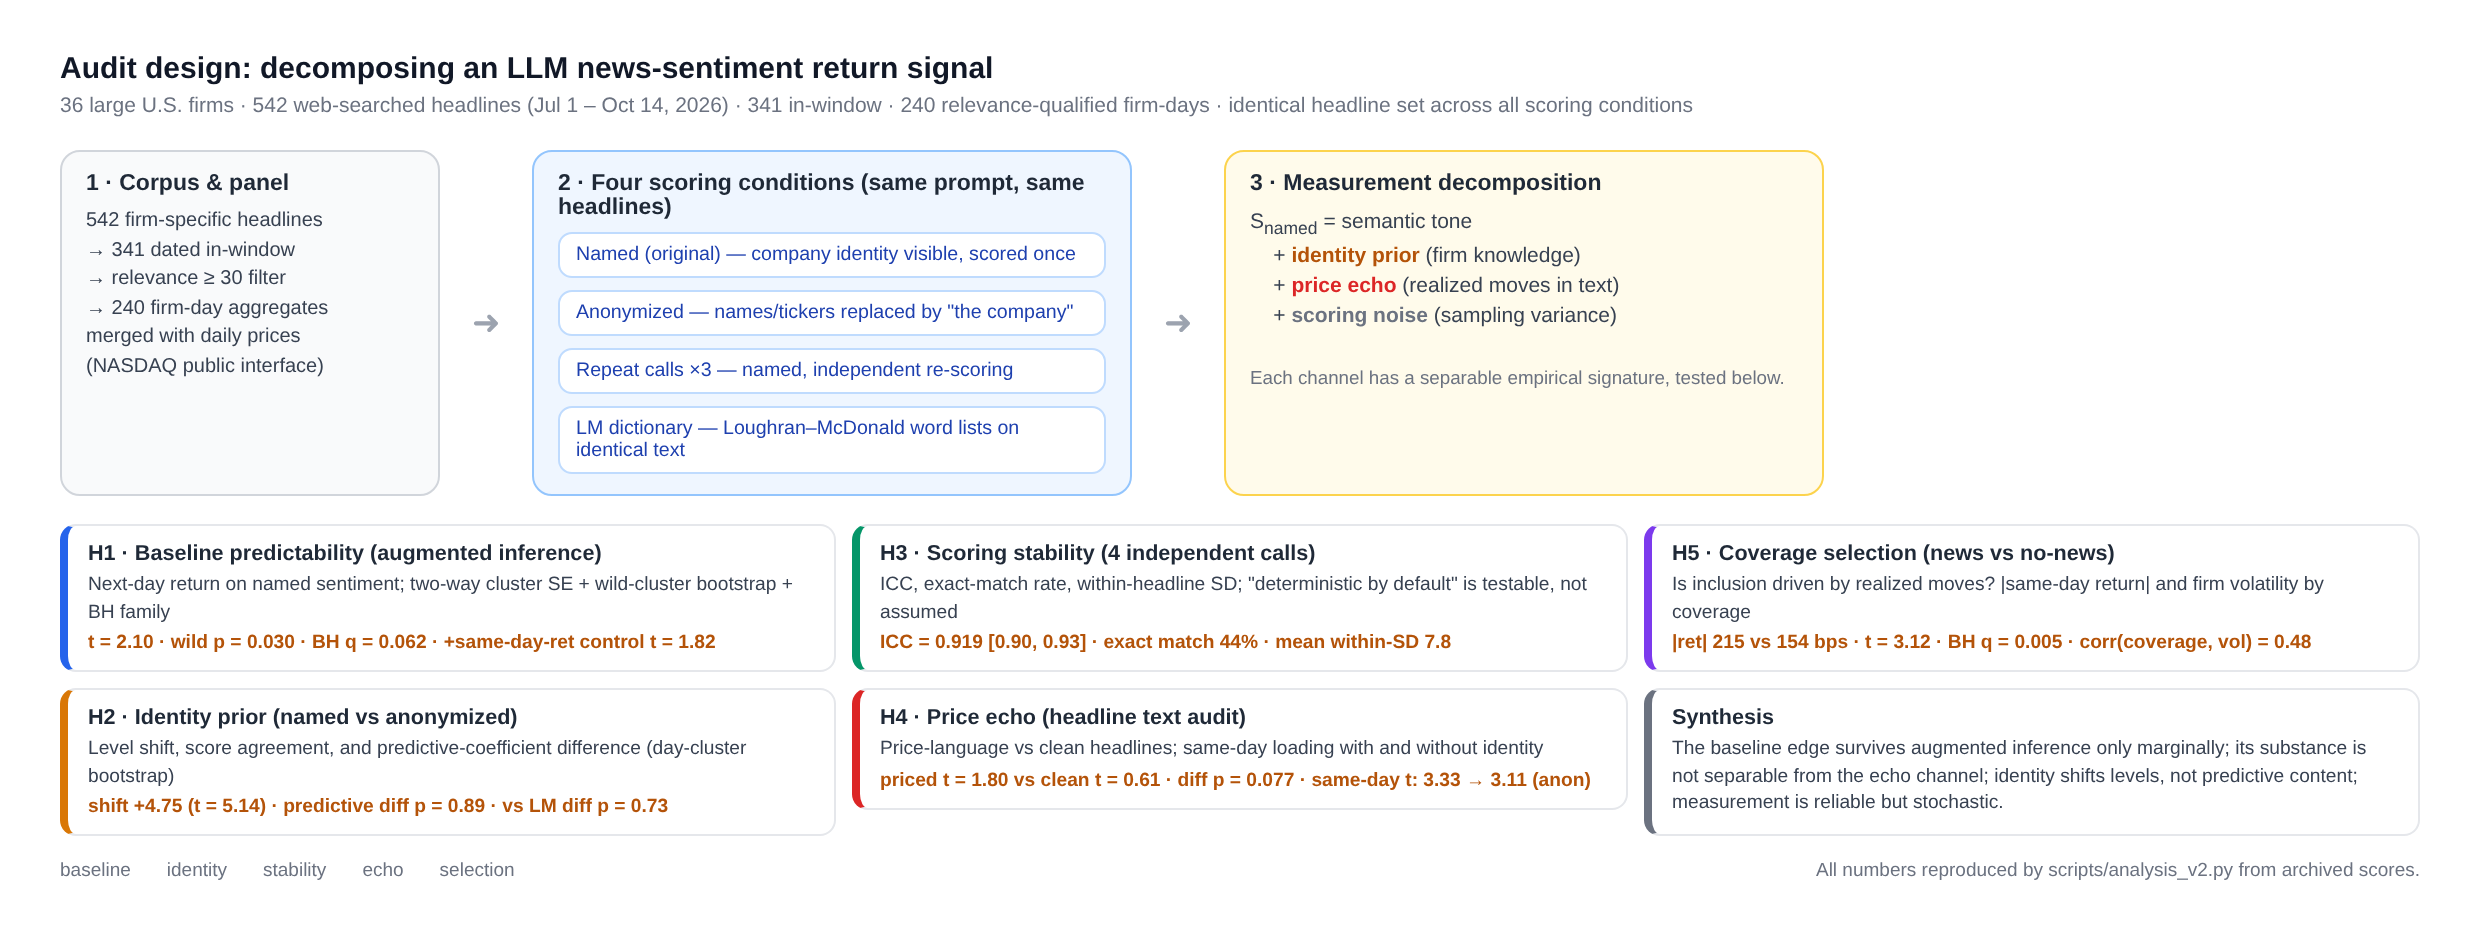
\includegraphics{../data/figures/fig_audit_design.png}
\end{adjustbox}
\caption{Audit design. One frozen corpus is scored under four conditions (named, anonymized, three repeat calls, dictionary), each isolating one term of the measurement decomposition $S=\kappa\theta+\iota G+\rho P+\varepsilon$; the five pre-specified hypotheses test the channels jointly under a common inference standard. All numbers are reproduced by \texttt{analysis\_v2.py} from archived scores.}
\label{fig:design}
\end{figure}

% ============ 5. Audit Results ============
\section{Audit Results}\label{sec:results}

\subsection{H1: baseline predictability under augmented inference}\label{sec:results:h1}

Table~\ref{tab:core} column (1) reports the pre-specified baseline: next-day close-to-close returns on named firm-day sentiment with controls, two-way clustered. The coefficient is $0.0149$ ($t=2.10$, $p=0.035$), i.e., a one-standard-deviation sentiment increase (0.36 on the $[-1,1]$ scale) is associated with a 54 \bps{} next-day return. Three augmentations discipline this number. First, the Rademacher wild-cluster bootstrap (day-level, null-imposed, $B=1{,}999$) gives $p=0.030$: the result is not an artifact of one or two trading days. Second, the Benjamini--Hochberg correction over the declared seven-comparison family raises the implied $q$-value to $0.062$: the headline baseline would not survive a 5\% FDR threshold. Third, adding the same-day return as a control~---motivated by the echo analysis below~---reduces the coefficient to $0.0141$ with $t=1.82$ ($p=0.069$); adding the overnight component as well gives $t=1.71$. The honest reading of H1 is \emph{marginal evidence, sensitive to specification, in a 205-observation sample}. The design's resolution is similarly bounded: at 80\% power, the minimum detectable next-day coefficient is $0.020$~---one-third larger than the estimate itself~---and the power of the test against the observed effect is $0.56$ (Appendix~\ref{app:power}).

For comparability with the literature, the same-day coefficient is $0.0283$ ($t=3.33$, $N=205$): sentiment co-moves with the return realized \emph{on} the news day. This co-movement is central to the echo analysis of Section~\ref{sec:results:h4}, which shows that the loading is a property of the text, not evidence about how prices form.

A final augmentation uses the full set of archived scoring draws of the same headlines: \emph{draw stability}. Re-estimating the identical H1 specification with every archived named draw~---fourteen independent passes plus the two within-condition means, spanning six sittings and both batch compositions (enumerated in Section~\ref{sec:robust})~---yields coefficients in $[0.0104,\,0.0161]$ and $t$-statistics in $[1.47,\,2.12]$, with both range endpoints set by individual passes (the October-16 single repeats individually run $t=2.12$, $1.76$, $1.68$). The point estimate is stable to well within its own standard error, but the \emph{nominal significance of H1 is draw-dependent}: the baseline draw sits at the favorable end of the range, and a pipeline that scored once on a different day would have reported $p$ between $0.05$ and $0.14$. We accordingly read H1 as \emph{borderline evidence with a stable point estimate}, which is exactly the resolution the power analysis of Appendix~\ref{app:power} predicts for a true effect of this size.

\begin{table}[htbp]
\centering
\small
\caption{Core audit regressions (dependent variable: next-day return unless noted)}
\label{tab:core}
\begin{threeparttable}
\begin{tabular}{lcccccc}
\toprule
 & (1) & (2) & (3) & (4) & (5) & (6) \\
 & Named & Named & Anon. & Dict. & Price-lang. & Clean \\
\midrule
Sentiment (named) & 0.0149$^{*}$ & 0.0141 & & & 0.0470 & 0.0033 \\
 & (2.10) & (1.82) & & & (1.80) & (0.61) \\
Sentiment (anonymized) & & & 0.0144 & & & \\
 & & & (1.78) & & & \\
Dictionary tone & & & & 0.0268 & & \\
 & & & & (1.00) & & \\
Same-day return & & 0.0306 & & & 0.0961 & $-$0.0211 \\
 & & (0.38) & & & (1.13) & ($-$0.29) \\
Controls & Yes & Yes & Yes & Yes & Yes & Yes \\
\midrule
$N$ & 205 & 205 & 205 & 205 & 38 & 167 \\
Wild-cluster bootstrap $p$ & 0.030 &~--- &~--- &~--- &~--- &~--- \\
BH family $q$ & 0.062 &~--- &~--- &~--- &~--- &~--- \\
\bottomrule
\end{tabular}
\begin{tablenotes}[flushleft]\footnotesize
\item All specifications include lagged return, lagged 21-day volatility, and the equal-weighted market return; $t$-statistics in parentheses, clustered by firm and trading day. Columns (5)--(6) split the sample by whether any headline for the firm-day contains realized-price language (15.2\% of headlines); both include the same-day return as a control. Wild-cluster bootstrap: Rademacher weights at the day level, null imposed, $B=1{,}999$. BH $q$: Benjamini--Hochberg FDR over the declared family of Table~\ref{tab:bh}. $^{*}$10\%, $^{**}$5\%, $^{***}$1\%.
\end{tablenotes}
\end{threeparttable}
\end{table}

Figure~\ref{fig:forest} presents all core coefficients with 95\% confidence intervals: the audit's message in one picture is that every instrument-condition coefficient is positive, every interval is wide, and the differences among them are the object of the next subsection.

\begin{figure}[htbp]
\centering
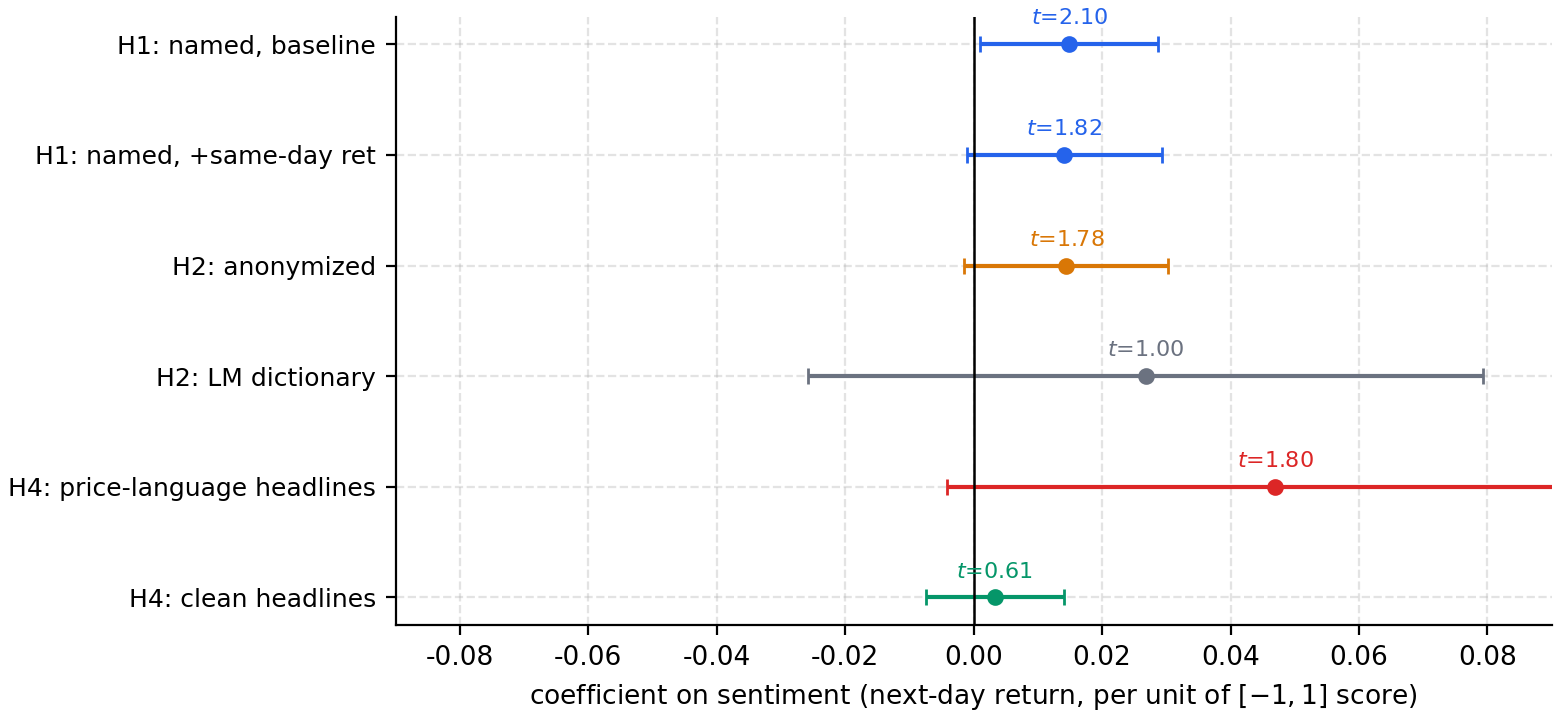
\includegraphics[width=0.92\textwidth]{../data/figures/fig_forest.png}
\caption{Core coefficients with 95\% confidence intervals (two-way clustered). No pairwise difference reaches conventional significance (Table~\ref{tab:diff}); the named, anonymized, and swapped conditions are formally equivalent at the half-benchmark margin, the dictionary comparison is inconclusive in both directions (Appendix~\ref{app:power}); the predictive loading is concentrated in price-language headlines.}
\label{fig:forest}
\end{figure}

\subsection{H2: de-identification shifts levels, not predictive content}\label{sec:results:h2}

\emph{The definitive estimate: a pre-specified, batch-interleaved design.} The identity contrast this paper reports was established by a third sitting (2026-10-18) that re-fielded both conditions under the protocol the audit ends up recommending: four rounds of the named protocol and four of the anonymized protocol over the identical 341 headlines, in a single sitting, with condition order alternated at the batch level (within each round, even-numbered batches of 25 call named-then-anonymized, odd-numbered call anonymized-then-named), protocol verbatim-identical, every call logged with timestamps and served-model identification (\texttt{glm-4-plus}). The design was pre-specified in an archived design document before any of its data was collected and is reported as a confirmatory contrast outside the declared family, well-powered under both headline-level and call-clustered inference. It establishes the identity level effect: $-2.82$ points in the named-minus-anonymized direction, with every one of the four round-level estimates negative ($-3.99$, $-2.05$, $-2.74$, $-2.51$; round-level $t=6.8$, $p=0.007$)~---\emph{anonymized scores sit systematically above their named twins by about three points}, a real but mild de-identification effect whose mechanism the fifth session's controls pin down below. One inference discipline applies here and below: because each API call returns all 25 scores of a batch in a single response, the scores of one call share a response-level \emph{mood} (Section~\ref{sec:results:h3} quantifies it at 13\% of residual variance), so headline-level paired tests overstate precision; under the most conservative clustering (14 batch-calls) the identity effect retains $t=2.7$ ($p=0.017$; 95\% CI $[-4.85, -0.79]$), and the estimate excluding the ten ticker-V headlines whose anonymization was a no-op (Appendix~\ref{app:anon}) is $-3.13$ with $t=4.8$ ($p=0.0003$). The order alternation makes call-order contamination testable: the effect is $3.34$ points (in the anonymized-minus-named direction) on batches where the named call came first versus $2.27$ where it came second~---similar magnitudes, no order artifact. The paired exact-match rate between interleaved condition calls is 48.5\%, bracketed by the within-condition repeat rates, exactly as a level displacement with stochastic noise predicts.

\emph{What the level effect is made of, and what it pools to.} A named-versus-anonymized contrast bundles two changes: the identity is removed, and the text is rewritten. Two pre-specified sittings separate the ingredients (2026-10-19 and 2026-10-25; design documents and falsifiable predictions archived before collection; Appendices~\ref{app:session5} and~\ref{app:session6}), and all contrasts below run under the locked analysis plans. \emph{Under corrected anonymization the contrast recurs}: with the ticker-V alias failure repaired and a forced verification pass reporting zero residual focal identifiers, the fifth sitting's named-minus-anonymized level difference is $-2.05$ points (headline-level $t=-2.84$, $p=0.005$; Wilcoxon $p<0.001$; under the conservative 14-cluster inference, $t=-1.36$, $p=0.18$), and the sixth sitting replicates it a third time (named minus anonymized $-2.54$, clustered $p=0.15$). Individually, only the interleaved session clears the conservative clustering, so the paper's summary number is the pooled one: across sessions 3, 5, and 6, a DerSimonian--Laird random-effects meta-analysis of the three call-clustered estimates ($-2.82$, SE 1.04; $-2.05$, SE 1.51; $-2.54$, SE 1.78) pools the de-identification effect at $-2.57$ points (95\% CI $[-4.08, -1.06]$, $z=3.34$; between-session heterogeneity nil: $\tau^2=0$, $I^2=0\%$). One caveat travels with the number: the three sessions re-score the same 341 headlines, and their per-headline responses correlate across sessions ($\rho=0.32$--$0.45$), so the three estimates are not independent draws; a conservative variant that adds those correlations to the full clustered standard errors widens the pooled interval to $[-4.56, -0.58]$~---still excluding zero (Appendix~\ref{app:session6}). \emph{The swap control does not support a material firm-specific prior}: replacing each headline's focal identifiers with a \emph{different} firm's identifiers~---natural text, wrong identity~---moves levels by $+0.34$ points against the named anchor ($t=0.40$, $p=0.69$; clustered $p=0.86$), far inside the repeat-noise floor, while the swapped condition sits $-2.39$ points below the anonymized one ($t=-3.26$, $p=0.001$; clustered $p=0.08$): the wrong firm's name sits with the right firm's name, two-plus points away from the placeholder. \emph{The prefix format is innocent}: adding a ``[Company X]'' prefix to the anonymized text moves levels by $+0.13$ (clustered $p=0.92$). \emph{A fictional-name control}~---scoring the identical 341 headlines with invented firm names, natural text, a concrete name, no real-world prior by construction~---places the fictional level almost exactly midway between named and anonymized (fictional minus named $+1.20$, clustered $p=0.45$; fictional minus anonymized $-1.33$, clustered $p=0.45$; the two clustered $p$-values are near-identical because the midpoint placement gives both sub-contrasts the same clustered $|t|$). Neither sub-contrast is individually established under clustered inference, so the split~---roughly half the displacement tied to the real name itself (identity associations or familiarity), half to the placeholder rewrite~---is a point-estimate reading rather than a certified decomposition. A leakage audit strengthens the swap contrast's reading: a transparent, data-driven cue lexicon flags 15.0\% of swapped headlines as still containing an original-firm lexical cue (26.7\% under a broader rule; six headlines, 1.8\%, retain the original identity outright through concatenated name variants such as ``ExxonMobil'' that the session-5 word-boundary verification cannot see), and excluding every flagged headline leaves the swap contrast at $+0.36$ to $+0.42$~---the null is not an artifact of identity leakage. The named-versus-anonymized level effect is therefore best read as a \emph{de-identification} effect~---removing the firm's real name raises scores, whoever the name belonged to~---with no support for a material prior about which firm the name denotes, and we use the accurate name throughout. The prediction layer agrees across every variant: the next-day coefficient is $0.0140$ (named), $0.0158$ (anonymized-v2), $0.0179$ (swapped), and $0.0134$ (prefixed; descriptive), with named-versus-anonymized and named-versus-swapped differences at $p=0.93$ and $p=0.92$~---de-identification moves levels, while the predictive coefficient stays formally equivalent at the half-benchmark margin. The formal level-layer equivalence battery at a pre-fixed margin of $\delta=1.25$ points (the prefix control certifies; the swap does not, minimum passing margin 1.73 points headline-level), the economics-anchored margins, and the session-by-session prediction-outcome tables are in Appendices~\ref{app:power}, \ref{app:session5}, and~\ref{app:session6}.


\emph{The superseded two-session benchmark.} The interleaved design exists because the original fielding~---named scores from 2026-10-15 against anonymized scores fielded twelve hours later~---read as a $+4.75$-point identity prior (paired $t=5.14$, $p<10^{-6}$), and the staged sessions then unraveled that reading: the named protocol itself drifted $+5.79$ points between the sittings, itself mostly batch composition, and the same-session residual~---a one-point displacement whose significance depended on the test and on the ticker-V exclusion~---was a range, not a verdict, which the interleaved design resolved at $-2.82$, opposite in sign to the naive shift. The full anatomy of the superseded benchmark~---distributional agreement, displacement magnitudes, the exact additive decomposition, the V-exclusion refinement, and the two figures that made the naive reading tempting~---is archived in Appendix~\ref{app:session} rather than carried in the main text, so the definitive interleaved estimate and its controls remain the only identity numbers a reader of the results must retain. The protocol lesson is general: condition contrasts fielded in separate sittings absorb session-level drift, and only same-session interleaving identifies the contrast the design intends.

\emph{What the drift is made of.} The interleaved session also closes the one question the two-session evidence could not answer: whether the $+5.79$ cross-session drift reflects the serving endpoint or the change in batch composition between sittings (session 1 scored the headlines embedded in the full 542-article stream; session 2 scored them alone). The October-18 sitting includes a control pass for exactly this: the \emph{identical} 341 headlines scored under the original 542-article batch composition, in the same session, same endpoint, same order. The composition effect is $+3.61$ points (headline-level paired $t=4.55$; batch-call-clustered $t=2.74$, $p=0.012$), and a fourth sitting re-ran the control with the run order \emph{inverted}~---composition pass first, 341-pass last, so that time-of-session works against the effect~---and reproduces it at $+3.50$ (clustered $t=2.17$); the pooled two-session estimate is $+3.56$ ($z=3.4$). Together with the two fixed-composition session legs, this gives an additive decomposition of the published drift: $+5.79 \approx +1.05$ (session 1 minus session 3, both at the 542 composition) $+\;3.61$ (composition, within session 3) $+\;1.14$ (session 3 minus session 2, both at the 341 composition), with the endpoint legs non-monotonic and the cross-session drift at fixed composition measuring $+0.56$ ($t=0.3$) between sessions 3 and 4. Batch composition, not endpoint change, carries roughly 62\% of the apparent ``session drift''~---which means the score of a headline depends measurably on \emph{which other headlines are scored alongside it}, a measurement-validity channel that, to our knowledge, has not previously been quantified in the LLM-finance setting; the NLP literature has documented the adjacent phenomena of batch-level accuracy loss and position/order sensitivity in batched prompting \citep{lin2024batch,liu2024lost,zheng2024}, but not their effect on the \emph{level} of a numeric measurement instrument. The fourth sitting also randomized the batch assignment of the 341 (seeded shuffle): re-batching the \emph{same} corpus moves levels by $+4.72$ points (clustered $t=2.02$, $p=0.065$~---suggestive). The mechanism accounting of Appendix~\ref{app:interleaved} bounds both shifts precisely, and neither lives in the linear part. Linear anchoring on batch-mates' fixed content is estimated at $\theta=+0.36$ ($t=4.9$; re-estimated with the full mate pool, $+0.38$, $t=5.0$), and for re-batching a \emph{fixed} corpus it \emph{provably} cannot shift the corpus mean (the telescoping identity: any re-partition preserves the average of leave-one-out batch-mate means). For the composition contrast the mate pool itself changes~---the 542-article batches seat each in-window headline next to out-of-window titles on 31\% of its batch-mate slots on average~---so there the linear component is quantifiable rather than barred: the 201 out-of-window titles average $-1.3$ points \emph{below} the in-window headlines they sit beside (35\% positive versus 62\%), and linear anchoring predicts a shift of $+0.04$ points against the observed $+3.56$~---about 1\%~---with full explanation requiring an out-minus-in content gap near $+30$ points, an order of magnitude beyond the actual gap and in the wrong direction. The estimated non-linearity does not close the residual either: asymmetric assimilation (positive batch-mates assimilate at $+0.69$, $t=2.3$; negative ones do nothing) would predict a small \emph{decrease}, because the added mates are less positive than those they replace. Both level shifts~---$+3.56$ from composition, $+4.72$ from re-batching alone~---therefore live almost entirely in response-level components that the current design does not separate: contrast-type responses to batch context, within-response position, and the mood shared by each response's 25 scores (Appendix~\ref{app:interleaved}, Table~\ref{tab:mech}). The mechanism is bounded, not closed, and we report it as such. A pre-registered batch-size dose-response session (a seeded 50-headline subsample scored alone, in fives, and in twenty-fives, one pass per size, within one sitting) leaves the presence channel open rather than closed: the singleton-versus-25 difference is $-0.20$ points ($t=-0.09$, $n=50$; SE $2.35$), so its 95\% CI of $[-4.92, +4.52]$ points cannot exclude a shift of the composition effect's own size~---an equivalence test would certify the singleton contrast only at a margin of $4.1$ points, wider than the effect itself~---and the same session carries an unexplained anomaly (the size-5 pass sits $5.5$--$5.7$ points below both neighbors, $t$ between $2.3$ and $2.5$) together with per-call noise SDs of 11--12 points across all three sizes that day, above the session-3 within-round benchmark of $7.2$ (Appendix~\ref{app:session6}). What the design establishes, under inverted run order, is that \emph{changed} mate composition moves levels; whether mere batch-mate presence also does is a question the dose-response leaves open. For pipelines the operational consequence is sharper than the session rule: hold the batch composition fixed across any comparison~---across conditions, sessions, or model versions~---because re-batching alone moves levels by more than the effect most studies are trying to measure.

\paragraph{Downstream consequences of the composition effect.} A natural objection: if levels move but slopes do not, what is the harm? The staged accounting over the archived sources of sessions 1--4 (all named protocol, identical 341 headlines; computed from archived draws, outside the declared family; \texttt{batch\_downstream.py}; full per-source accounting in Appendix~\ref{app:interleaved}) carries the operational verdict. Slopes and ranks are robust: the predictive coefficient stays in $[0.010, 0.016]$ across all seven sources, every composition and re-batch contrast of slopes is insignificant ($p>0.9$), and the cross-sectional ranking of firm-days correlates at $\rho\geq 0.81$ across compositions (0.97 at fixed composition across sessions). Absolute-scale uses are not robust: between the two compositions of the same session, a fixed ``score $\geq +50$'' filter more than doubles its trade count (22 to 50 firm-days in session 3; 27 to 43 in session 4), the daily-mean series shifts by 4.0--4.6 points, and the sign of the day-over-day change in daily sentiment flips on 16--24\% of trading days. The composition effect is therefore a \emph{level} pathology with boundary costs: harmless to conditional, cross-sectional, and regression uses in this sample, and disqualifying for threshold rules, absolute-score comparisons across pipelines, and time-series signals built on the score's level; Table~\ref{tab:downstream} and Figure~\ref{fig:downstream} itemize the accounting (Appendix~\ref{app:interleaved}).

\emph{Prediction layer.} The named-versus-anonymized predictive difference is tested three ways and never approaches significance: cross-session ($0.0004$, 95\% CI $[-0.0044, 0.0045]$, $p=0.887$), inside the October-16 sitting ($0.0002$, $p=0.905$), and interleaved inside October-18 ($+0.0013$, 95\% CI $[-0.0034, 0.0074]$, $p=0.622$)~---no difference is detected, which, as Section~\ref{sec:framework:inference} stresses, is not yet evidence of equivalence. Every instrument contrast is therefore re-assessed as a formal two-one-sided-tests (TOST) equivalence assessment at a margin of $\delta^{*}=0.0074$~---half the benchmark coefficient, about 27 \bps{} of next-day response per one-standard-deviation sentiment shock~---using the day-cluster bootstrap's 90\% interval as the test statistic and reporting each contrast's minimum passing margin so that any reader-preferred margin can be tested directly (Appendix~\ref{app:power}; exploratory, outside the declared family). The verdict upgrades some conclusions and bounds others. \emph{Upgraded}: all four named-versus-anonymized contrasts~---cross-session, same-session, interleaved, and the fifth session's corrected variant~---are formally equivalent at $\delta^{*}$, their 90\% intervals closing at 21--42\% of the benchmark coefficient (power 0.74--0.99 against a true difference of zero), so instrument invariance under de-identification is now an equivalence finding, not a failure to find. \emph{Bounded}: the swap contrast is the one near-miss~---its interval $[-0.0083, +0.0004]$ requires a margin of 0.0083, 56\% of the benchmark~---and the dictionary comparison is uninformative in \emph{both} directions: its interval $[-0.0658, +0.0415]$ fits no defensible margin ($4.4\times$ the benchmark, zero power, a hundredfold-plus sample needed), so this sample can establish neither that the LLM and the dictionary differ nor that they agree, and the earlier rhetorical question of which instrument ``wins'' is not answerable here. The verdicts are also margin-specific, and the benchmark-anchored margin is itself the weakest link~---the benchmark $t$ ranges over $[1.47, 2.12]$ across draws~---so Appendix~\ref{app:power} re-evaluates the battery at a stricter, economics-anchored margin of 10 \bps{} of next-day response per one-standard-deviation sentiment shock, a round threshold independent of the benchmark coefficient: no contrast passes (minimum passing margins run 11.5--29.8 \bps/SD across the four de-identification contrasts and the swap; the dictionary needs 237), and 3.6--7.8 times the sample would be required for 80\% power there, so the equivalence findings should be read as bounded at roughly a fifth to half of the benchmark effect rather than certified at arbitrary precision. The sixth session's prediction layer agrees across all three of its conditions ($\beta=0.0126$ named, $0.0112$ anonymized, $0.0113$ fictional; every pairwise difference $p\geq 0.62$). In a horse race on the same observations (not shown to avoid triple-counting), both coefficients remain individually insignificant at 5\%, which is exactly what low power plus attenuation predicts (Remark~\ref{prop:attenuation}, clause~(iii)).

\begin{table}[htbp]
\centering
\small
\caption{Formal difference tests (day-cluster bootstrap, $B=999$)}
\label{tab:diff}
\begin{threeparttable}
\begin{adjustbox}{max width=\textwidth}
\begin{tabular}{lccc}
\toprule
Contrast & Observed difference & 95\% CI & $p$-value \\
\midrule
$\beta_{\text{named}}-\beta_{\text{anonymized}}$ (cross-session) & 0.0004 & $[-0.0044,\ 0.0045]$ & 0.887 \\
$\beta_{\text{named}}-\beta_{\text{anonymized}}$ (same session) & 0.0002 & $[-0.0034,\ 0.0037]$ & 0.905 \\
$\beta_{\text{named}}-\beta_{\text{anonymized}}$ (interleaved) & 0.0013 & $[-0.0034,\ 0.0074]$ & 0.622 \\
$\beta_{\text{named}}-\beta_{\text{dictionary}}$ & $-$0.0119 & $[-0.0737,\ 0.0576]$ & 0.731 \\
$\beta_{\text{price-lang.}}-\beta_{\text{clean}}$ & 0.0436 & $[-0.0059,\ 0.1105]$ & 0.100 \\
Level shift, cross-session (points) & $+$4.75 &~--- & $<$0.0001 \\
Session drift (points) & $+$5.79 &~--- & $<$0.0001 \\
Identity, same session (points) & $-$1.04 & $[-2.32,\ +0.23]$ & 0.111 \\
Identity, same session, excl.\ V (points) & $-$1.29 & $[-2.53,\ -0.05]$ & 0.041 \\
Identity, interleaved sess.\ 3 (points) & $-$2.82 & $[-4.85,\ -0.79]$ & 0.017 \\
\quad excl.\ ticker V & $-$3.13 & $[-4.41,\ -1.86]$ & 0.0003 \\
De-identification, sess.\ 5, corrected anon.\ (points) & $-$2.05 &~--- & 0.175 \\
Identity swap vs.\ named, sess.\ 5 (points) & $+$0.34 &~--- & 0.857 \\
Composition effect, sess.\ 3 (points) & $+$3.61 & $[+1.03,\ +6.20]$ & 0.012 \\
Composition effect, sess.\ 4, order inverted & $+$3.50 &~--- & 0.042 \\
Re-batch (random), sess.\ 4 & $+$4.72 &~--- & 0.065 \\
Fictional minus named, sess.\ 6 (points) & $+$1.20 &~--- & 0.450 \\
Fictional minus anonymized, sess.\ 6 (points) & $-$1.33 &~--- & 0.450 \\
Identity (de-identification), sess.\ 6 (points) & $-$2.54 &~--- & 0.153 \\
Identity, pooled sess.\ 3/5/6, random effects & $-$2.57 & $[-4.08,\ -1.06]$ & 0.001 \\
Batch size 1 vs.\ 25, sess.\ 6b ($n=50$, points) & $-$0.20 & $[-4.92,\ +4.52]$ & 0.93 \\
\bottomrule
\end{tabular}
\end{adjustbox}
\begin{tablenotes}[flushleft]\footnotesize
\item Differences of next-day predictive coefficients from Table~\ref{tab:core} specifications; bootstrap resamples trading-day clusters ($B=999$; the price-language row uses $B=9{,}999$ under the same-day-control specification actually estimated, and is seed-stable: three independent seeds give $p$ between 0.093 and 0.100; the interleaved row uses $B=9{,}999$). Level rows are paired $t$-tests at the article level ($n=341$, points on the $[-100,100]$ scale): cross-session rows compare the 2026-10-15 named round with the 2026-10-16 round; the same-session identity rows compare the anonymized condition against the mean of the three October-16 named repeats. The last eight rows are staged confirmatory contrasts of the interleaved and control sessions (2026-10-18, a mechanism sitting, and 2026-10-19; Sections~\ref{sec:results:h2} and Appendix~\ref{app:interleaved}), each pre-specified in an archived design document before its data collection, reported outside the declared family, and evaluated under batch-call-clustered inference because the 25 scores of one API response share a response-level mood (13\% of residual variance; Section~\ref{sec:results:h3})~---headline-level tests of the same contrasts give $t=4.28$ (identity), $t=4.55$ (composition), and $t=-2.84$/$t=0.40$ (session-5 de-identification/swap), and the round-level identity meta-test gives $t=6.8$ ($p=0.007$). The V exclusion drops the ten headlines whose anonymization was a no-op (Appendix~\ref{app:anon}); the composition rows compare the identical 341 headlines scored inside the original 542-article batches versus the 341-only batches of the same session (session 4 with the run order inverted); the re-batch row compares seeded-random batches to the standard order. ``One significant, the other not'' never appears in this table by construction: all cross-instrument statements are direct difference tests. Computed by \texttt{analysis\_v2.py} (family rows), \texttt{revision\_power.py} and \texttt{v\_exclusion.py} (session rows), \texttt{analysis\_v3.py} / \texttt{analysis\_v4.py} / \texttt{reinference.py} (session-3/4 rows), and \texttt{analysis\_v5.py} (session-5 rows); the session-6 and batch-size rows are computed by \texttt{analysis\_v6.py} and \texttt{analysis\_v6b.py} under the same conventions (the batch-size row is a headline-level test on the 50-title subsample, where call clustering is degenerate), with level-layer equivalence margins from \texttt{level\_tost\_and\_margins.py} and the swapped-text leakage audit from \texttt{swap\_leakage\_audit.py} (Appendix~\ref{app:session6}). The pooled row is a DerSimonian--Laird random-effects meta-analysis of the three session-level clustered estimates, treating sessions as independent; because the sessions re-score the same 341 headlines, a conservative variant that applies the empirical cross-session correlation of per-headline responses ($\rho=0.32$--$0.45$) to the full clustered standard errors widens its interval to $[-4.56, -0.58]$ (\texttt{meta\_deident\_pooling.py}, \texttt{results\_meta\_deident.json}). The batch-size row's interval is the headline-level paired $t$ interval on the 50-title subsample.
\end{tablenotes}
\end{threeparttable}
\end{table}

The two-layer result is the paper's cleanest inference about what the model brings to the text~---corrected by its own staged designs and confirmed by the interleaved experiment, then re-attributed by the swap control: de-identification moves the level by $-2.6$ points pooled across three sessions (named scores sit \emph{below} their anonymized twins; the wrong firm's name sits with the right one), batch composition moves levels by another three-plus points, and the predictive signal they leave behind is formally equivalent at the half-benchmark margin in every de-identification contrast, with the swap contrast equivalent only at a 56\% margin (Appendix~\ref{app:power}). A displacement that raised all of a firm's headlines equally would be differenced out of any predictive regression that conditions on the firm; a displacement that differentially tracked which headlines \emph{matter} would have shown up as a predictive difference, and does not. The level evidence that initially pointed the other way measured the session and the batch, not the displacement~---and the sign it hid was the opposite of the naïve reading.

\subsection{H3: the instrument is reliable but stochastic}\label{sec:results:h3}

Four independent calls of the identical prompt on the identical headlines yield an intra-class correlation $\text{ICC}(2,4)=0.919$ with a bootstrap 95\% CI of $[0.90, 0.93]$; mean pairwise Pearson correlation across draws is $0.928$; 29.9\% of headlines receive the identical score in all four calls (44.0\% for the original-versus-draw-1 pair alone), and the mean within-headline standard deviation is 7.8 points (Figure~\ref{fig:reliability}). Those four calls span two sittings; the three October-16 draws alone give $\text{ICC}(2,3)=0.949$, so pooling across the twelve-hour gap costs three reliability points. The interleaved session answers the follow-up: Four October-18 named rounds give $\text{ICC}(2,4)=0.949$ with a within-headline standard deviation of 7.2 points (6.6 for the three October-16 rounds), and the interleaved anonymized rounds match (0.949): reliability is a stable property of the instrument, not of a particular sitting, even while the \emph{level} moves by points between the same sittings. The eight passes of the interleaved design also let the noise itself be decomposed, and the decomposition revises the intuition a single-repeat design encourages: 13\% of the residual variance is a \emph{response-level mood}~---a random level shared by all 25 headlines of one API response (SD $\approx2.6$ points)~---and only the remaining 87\% is idiosyncratic per headline per response (SD $\approx6.7$). Scoring is not 341 independent draws per pass but 14 correlated clusters, which is why the level contrasts of Section~\ref{sec:results:h2} are reported under call-clustered inference and why a pipeline that averages multi-headline batches inherits a noise floor its headline-level statistics hide. The pre-specified temperature-zero rounds of the fifth session close the loop on decoding settings: two identical named passes at \texttt{temperature}$\,=0$ return bitwise-identical scores for 83.3\% of headlines (284 of 341; within-headline SD 4.8 versus 7.2 under default decoding; mean absolute difference 2.4)~---substantially tighter, but 57 of 341 headlines still move between two calls at temperature zero, a pattern consistent with server-side nondeterminism that survives the decoding fix; the noise floor behaves as a property of the serving stack rather than of sampling settings alone. The temperature-zero level sits $+1.06$ points above the same-sitting default-decoding named level ($p=0.052$, two-sided, as pre-specified). The pooled number remains the right one for a production pipeline~---single-sitting ICCs overstate what re-scoring tomorrow will deliver~---which is also why the pooled ICC prices in the session drift of Section~\ref{sec:results:h2}. Reliability of $0.92$ is high by psychometric standards for a single-item instrument, and the mean-level agreement across draws (within one point) rules out gross instability. But it is emphatically \emph{not} determinism: a research pipeline that scores each headline once and treats the result as ``the'' score embeds a measurement-noise floor of $\pm8$ points per headline into every downstream construct. Under Remark~\ref{prop:attenuation}(i), the observed coefficient is attenuated by roughly the reliability ratio; with firm-day averaging over 1.25 headlines the attenuation is modest, which is the arithmetic reason the named and anonymized coefficients survive as similar point estimates. The practical implication is procedural: single-call scoring should report an ICC or repeat-call dispersion alongside any predictability statistic, and pipelines should score at least twice and average when headlines are cheap relative to inference~---as they are here.

\begin{figure}[htbp]
\centering
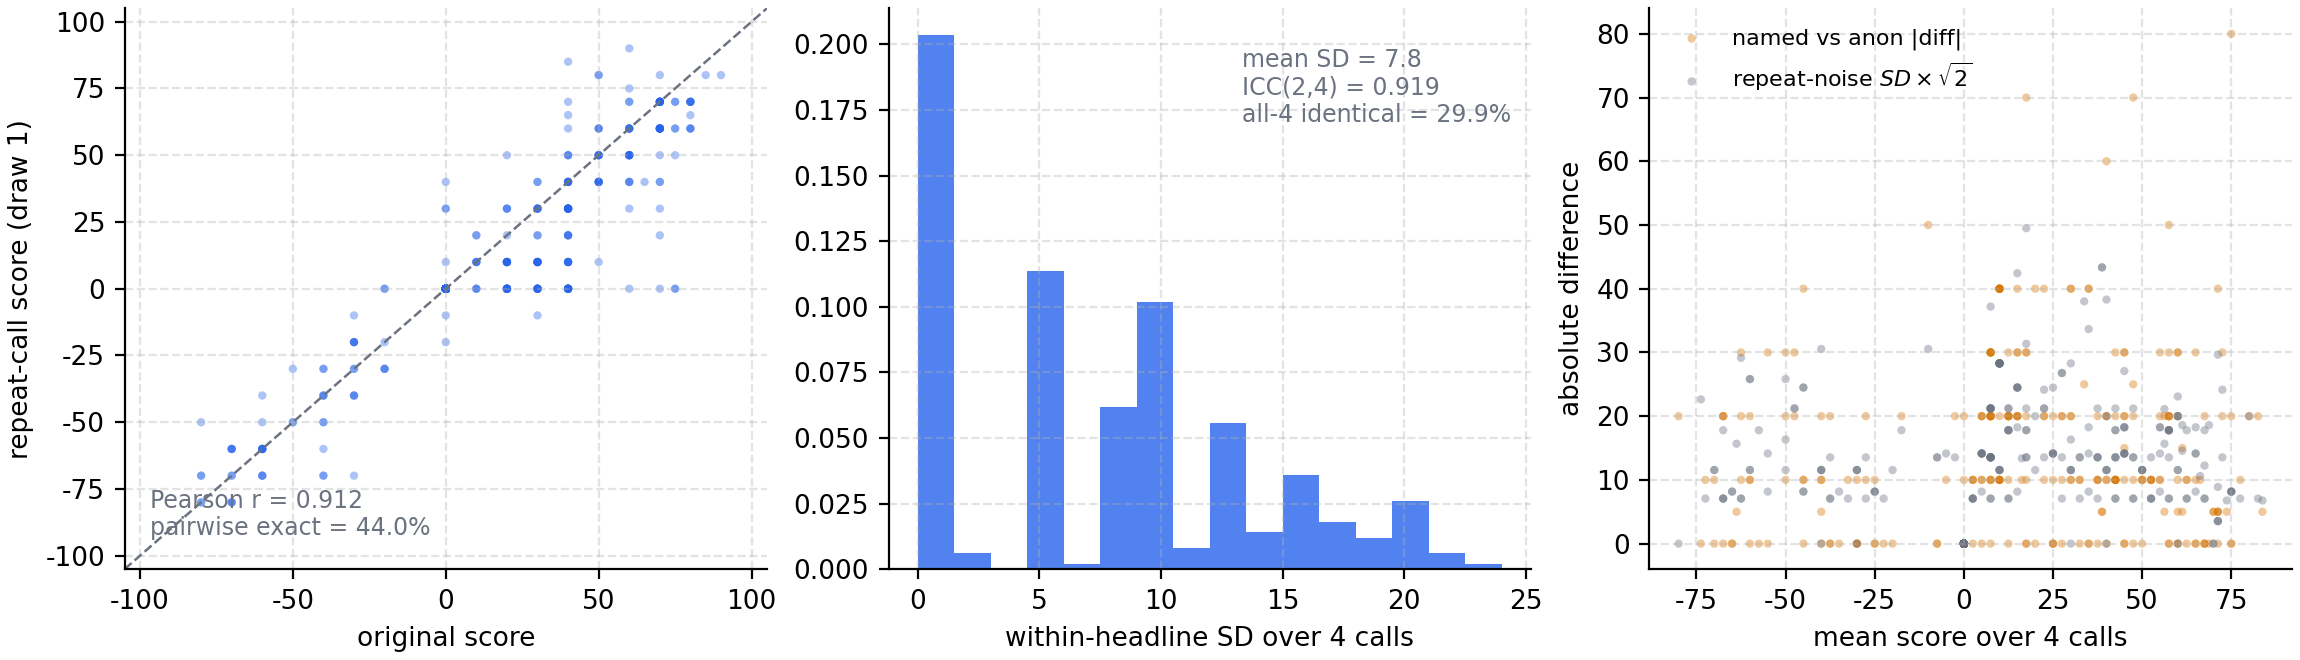
\includegraphics[width=\textwidth]{../data/figures/fig_reliability.png}
\caption{Repeat-call reliability. Left: original versus draw-1 scores ($r=0.912$; 44.0\% of the pair identical). Middle: within-headline standard deviation over four calls (mean 7.8 points); 29.9\% of headlines receive one identical score in all four calls. Right: Bland--Altman comparison of the named-versus-anonymized absolute difference against the repeat-noise floor ($\sqrt{2}\times$ within-SD): anonymization displaces scores by more than re-calling the model does.}
\label{fig:reliability}
\end{figure}

\subsection{H4: the predictive content sits in the price echo}\label{sec:results:h4}

A text audit flags headlines containing realized-price language~---movement verbs and magnitude constructions (``rose,'' ``surged,'' ``dropped by 5\% after earnings,'' ``up 20\% in 2026'')~---covering 52 of 341 in-window headlines (15.2\%). Table~\ref{tab:core} columns (5)--(6) split the firm-day sample by the flag (all specifications include the same-day return as a control): the coefficient is $0.047$ ($t=1.80$, $N=38$) for firm-days with price-language headlines and $0.003$ ($t=0.61$, $N=167$) without. The bootstrap difference is $0.044$ with 95\% CI $[-0.006, 0.110]$, $p=0.100$ ($B=9{,}999$, seed-stable; Table~\ref{tab:diff}): directional evidence~---underpowered in the tails and not clearing the 10\% threshold~---that the predictive loading concentrates where the text describes realized moves. On the magnitudes: the clean subsample's coefficient is one-fourteenth of the price-language coefficient ($0.003$ versus $0.047$) and about one-fifth of the baseline ($0.22$), insignificant~---but not established as \emph{equivalent} to zero: its 90\% interval reaches $0.0136$, 91\% of the benchmark (Appendix~\ref{app:power}), so this sample cannot separate ``no clean signal'' from ``a clean signal almost as large as the baseline.'' Essentially the entire point estimate of the baseline coefficient comes from the 19\% of the sample flagged as echoes.

Because the split's validity rests on a regular-expression classifier, we audited the classifier itself: all 52 flagged headlines were re-classified one by one against a written rulebook distinguishing realized price moves from fundamental-magnitude language, directional forecasts, and regex false positives. The classification is LLM-assisted and disclosed as such~---an internal audit of the flag, not independent human annotation (Appendix~\ref{app:classification}). The verdict: 43 of 52 (82.7\%) are genuine realized-price headlines, and re-running the split with only the strict realized-price firm-days leaves the point estimate essentially unchanged ($0.0475$ versus $0.0470$; $t=1.61$, $N=33$)~---the flag was noisy at the margin but not wrong where it mattered. The classification also sharpens the echo signature itself: strict-price firm-days average 361 \bps{} of absolute same-day return against 178 for clean days, while the nine misclassified headlines' firm-days average 120 \bps{}, below even the clean baseline. Leave-one-out and leave-one-company-out jackknifes of the priced-minus-clean difference keep every replicate positive (sign-flip rate 0.0; Appendix~\ref{app:classification}). The honest reading of H4 is unchanged by the audit~---directional, underpowered, text-located~---but it is now directional evidence whose classifier has itself been audited.

Two corroborating facts identify the channel as textual rather than mnemonic. First, the same-day loading of returns on sentiment is $t=3.33$ named and $t=3.11$ anonymized: if the same-day co-movement were driven by the scorer's memory of price outcomes, removing identity should have collapsed it; it barely moves. Second, the horizon path~---positive at $t+1$, negative at $t+2$ ($t=-2.04$)~---is exactly what short-horizon continuation-and-reversal around high-absolute-return events produces mechanically \citep{chan2003}, on a sample that (per H5) over-weights exactly those events. A reversal of this shape invites an attention-driven overshooting reading, but it is better read as the echo channel propagating through return dynamics; Section~\ref{sec:appaux} returns to this in the auxiliary analyses.

\begin{figure}[htbp]
\centering
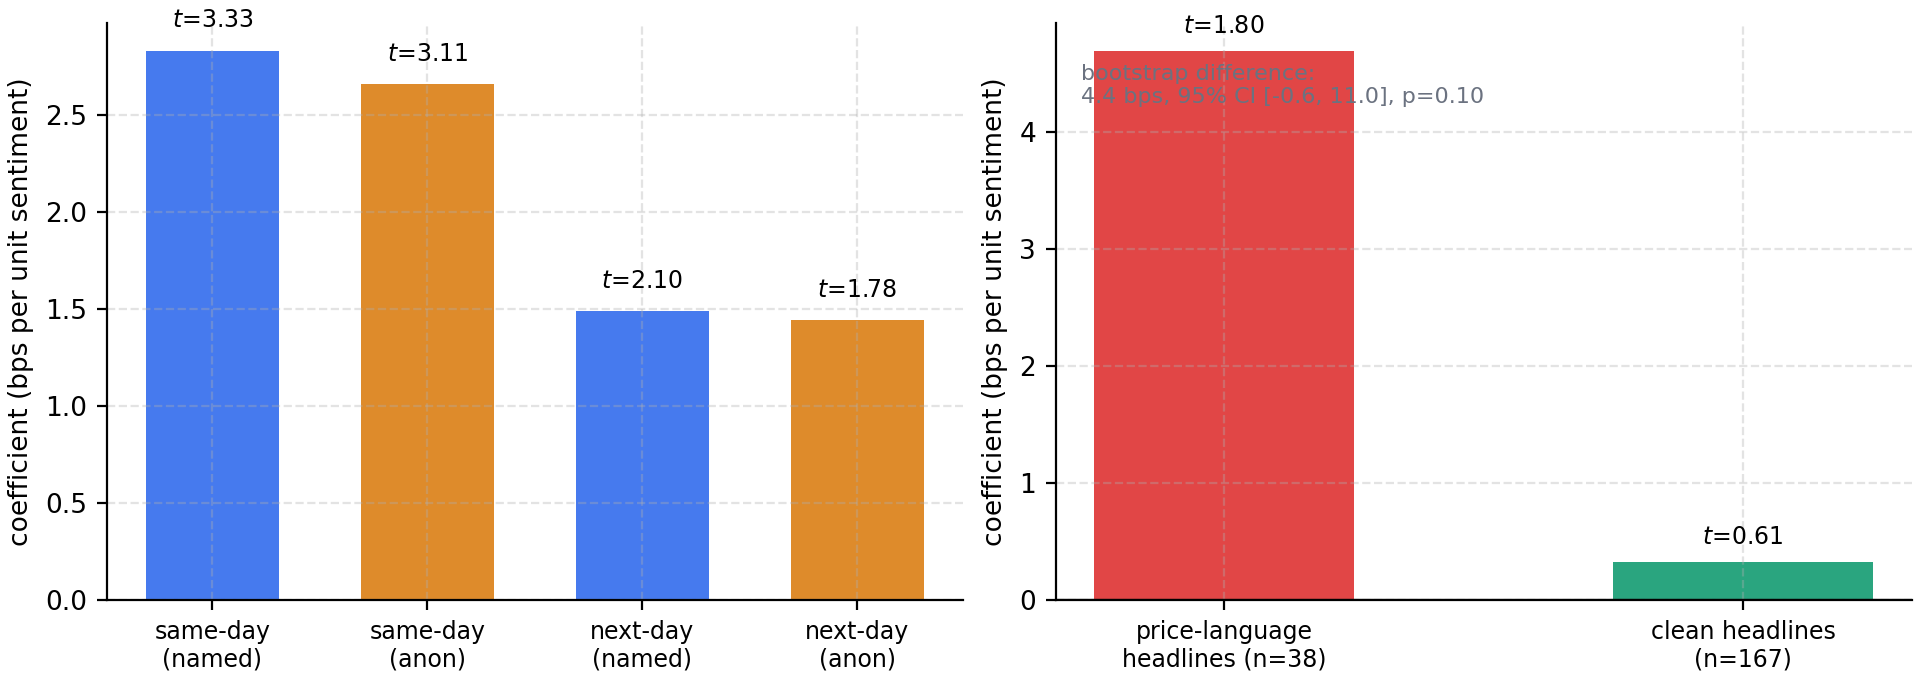
\includegraphics[width=\textwidth]{../data/figures/fig_echo.png}
\caption{The echo channel. Left: same-day and next-day coefficients, named versus anonymized~---anonymization does not remove the same-day loading (3.33 vs.\ 3.11), locating the contamination in the text. Right: next-day coefficients for price-language versus clean headlines, with the bootstrap difference.}
\label{fig:echo}
\end{figure}

\subsection{H5: coverage is selected on realized activity}\label{sec:results:h5}

Covered firm-days exhibit mean absolute same-day returns of 215 \bps{} against 154 \bps{} for uncovered firm-days, and firm-level news counts correlate 0.48 with firm return volatility (Figure~\ref{fig:selection}). A pooled two-sample statistic would pronounce this gap overwhelming ($t=3.12$, $p=0.002$), but it ignores the double indexing of the 2,664-cell panel~---the same firm repeats across days, and all firms share each trading day's market shock~---so the primary inference is a firm-and-day fixed-effects regression of absolute returns on the coverage indicator, estimated on the 2,628 firm-days with a non-missing same-day return (2,664 less the 36 first-trading-day cells, which lack a prior close), with two-way clustered standard errors: $t=2.76$ ($p=0.006$; BH $q=0.014$). Two robustness specifications agree: firm fixed effects with day-clustered errors give $t=2.49$ ($p=0.013$), and a day-cluster bootstrap of the gap gives $p\leq 0.002$ with 95\% CI $[25, 103]$ \bps. The selection equation~\eqref{eq:selection} is therefore rejected with $\delta_1>0$ under panel-appropriate inference: the audit sample over-weights high-activity events. It might be tempting to argue that coverage is driven by query design rather than by return outcomes, and that the consequence is statistical power rather than bias. That argument is wrong: search-driven collection selects on exactly the outcomes that make short-horizon continuation and reversal strongest for non-semantic reasons. The correction does not invalidate within-covered-sample inference, but it bounds external validity~---the estimand is the conditional (event-sampled) relationship, not the population relationship~---and it interacts with H4: high-activity events are both more likely to be covered and more likely to be covered \emph{retrospectively}.

\begin{figure}[htbp]
\centering
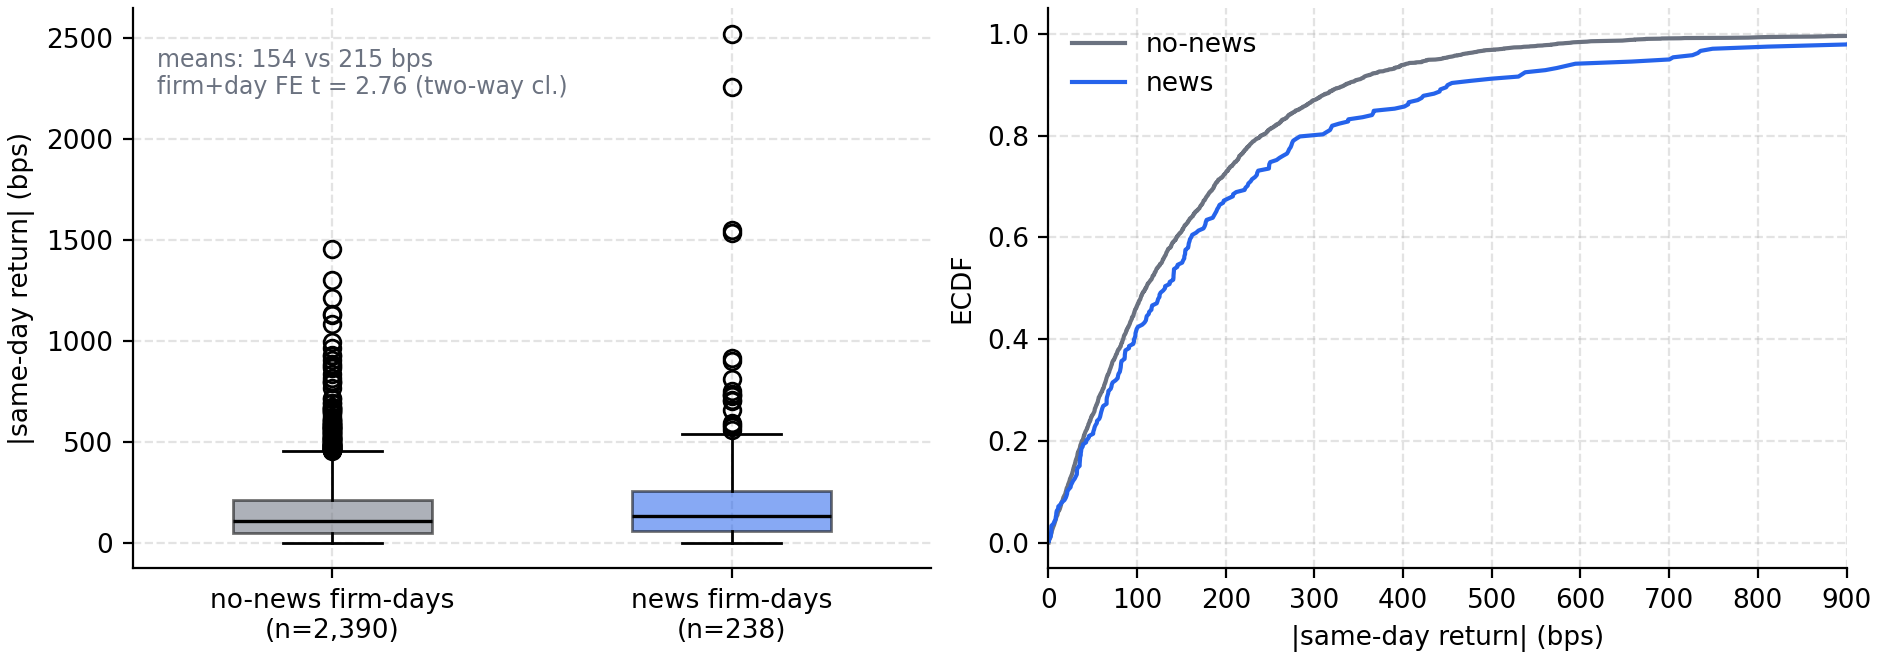
\includegraphics[width=0.95\textwidth]{../data/figures/fig_selection.png}
\caption{Coverage selection. Left: distribution of absolute same-day returns for covered versus uncovered firm-days. Right: empirical CDFs. Covered firm-days are drawn disproportionately from high-absolute-return states.}
\label{fig:selection}
\end{figure}

\subsection{Multiple-testing summary}

Table~\ref{tab:bh} reports the declared family with raw and Benjamini--Hochberg $q$-values. Three comparisons survive at any conventional threshold~---the named-versus-anonymized level shift ($q<0.0001$), the coverage-selection test ($q=0.014$), and the reliability ICC ($q<0.0001$, one-sided). The first of these requires re-interpretation rather than rejection: the level-shift test rejected because its contrast mixes an identity effect with a twelve-hour session gap, and the session component alone ($+5.79$, $t=7.03$) would clear any threshold; it survives as evidence of \emph{scoring instability across sittings}, not of an identity prior (Section~\ref{sec:results:h2}). The two channels that would constitute ``an LLM sentiment return signal''~---the baseline coefficient and its echo decomposition~---sit at $q=0.062$ and $q=0.140$ respectively. The pattern is itself informative: the audit finds the contamination and instability channels with confidence and the predictive content only marginally. The staged confirmatory contrasts of Section~\ref{sec:results:h2}~---the interleaved identity effect (round-level $p=0.007$; call-clustered $p=0.017$), its V-excluded variant ($p=0.0003$), the batch-composition effect (pooled $z=3.4$, two sessions with inverted run order), and the fifth session's swap and temperature-zero controls (Appendix~\ref{app:session5})~---sit outside the declared family by construction (they post-date it), but each was pre-specified in an archived design document before its data collection and they point the same way: the channels the audit measures with confidence are the ones the score carries for reasons other than the text's semantics.

\begin{table}[htbp]
\centering
\small
\caption{Declared test family: raw $p$-values and Benjamini--Hochberg $q$-values}
\label{tab:bh}
\begin{tabular}{lcc}
\toprule
Comparison & raw $p$ & BH $q$ \\
\midrule
H2: identity level shift (named $-$ anonymized) & $<$0.0001 & $<$0.0001 \\
H3: ICC $>$ 0.5 (one-sided bootstrap) & $<$0.0001 & $<$0.0001 \\
H5: coverage selection (firm+day FE, two-way cl.) & 0.0059 & 0.0137 \\
H1: baseline next-day coefficient (named) & 0.0354 & 0.0620 \\
H4: price-language vs.\ clean difference & 0.1002 & 0.1402 \\
H2: predictive difference, named vs.\ anonymized & 0.8869 & 0.8869 \\
H2: predictive difference, named vs.\ dictionary & 0.7307 & 0.8525 \\
\bottomrule
\end{tabular}
\begin{tablenotes}[flushleft]\footnotesize
\item Family declared in Section~\ref{sec:data} prior to augmented inference. The three rejections are measurement-layer channels; the two return-layer channels are marginal. $q$-values from the Benjamini--Hochberg step-up procedure at $m=7$. The H2 level-shift row compares conditions fielded twelve hours apart; Section~\ref{sec:results:h2} attributes most of it to between-session drift, and the same-session contrast ($p=0.11$, or $p=0.04$ excluding the ticker-V no-op anonymization) is a staged addition outside the declared family. The H5 row is the panel specification (firm and day fixed effects, two-way clustered; $N=2{,}628$ firm-days with non-missing same-day returns) that respects the panel's double indexing.
\end{tablenotes}
\end{table}

% ============ 6. Robustness and Threats to Validity ============
\section{Robustness and Threats to Validity}\label{sec:robust}

\subsection{Specification robustness of the baseline}

Five checks, all computed fresh on the archived data. (i)~Raising the relevance threshold from 30 to 50 leaves the baseline essentially unchanged ($t=2.12$, $N=187$). (ii)~Using the unweighted mean over all headlines with no relevance filter gives $t=2.07$ ($N=209$): the filter is not doing the work. (iii)~Dropping dense event days (five or more covered firms) leaves the point estimate intact but the statistic at $t=1.61$ ($N=117$): about a quarter of the baseline's strength comes from clustering on event days, consistent with H5. (iv)~The anonymized condition with the same-day control runs at $t=1.59$, tracking its named twin. (v)~A within-day permutation placebo (1{,}000 draws, sentiment permuted inside each trading day) yields a two-sided permutation $p=0.007$: whatever the baseline coefficient is, it is not an artifact of arbitrary re-labeling. The consistent picture across (i)--(v) is a real but fragile association~---robust to measurement choices, weakened by event-day down-weighting, and significant at conventional levels only under the original sample construction.

\subsection{Session robustness of the predictive coefficient}

The baseline coefficient rests on October-15 scores; the three October-16 named repeats re-score the identical headlines in a different sitting, the October-18 interleaved session re-scores them twice more per condition in a third, and the session-4 mechanism passes add three further named draws at both batch compositions plus a random re-batch. Across the fourteen archived named draws~---twelve individual passes (the original, three October-16 repeats, four October-18 rounds, the October-18 542-composition pass, and the three session-4 passes) plus the two session means~---the next-day coefficient lives in $[0.010, 0.016]$ and the $t$-statistic in $[1.47, 2.12]$: the point estimate is stable across sessions, compositions, and re-batching to well within its own standard error, and every repeat falls inside the range the specification checks above already span~---but the \emph{significance} of the coefficient moves with the draw, from $p=0.035$ (the baseline round) to $p=0.14$ (the weakest October-18 round). The same-day loading is large under every draw ($t$ between $2.96$ and $3.80$ for the session-1/2 draws). Session drift and batch composition are therefore \emph{level} phenomena~---they move the mean score by points (Section~\ref{sec:results:h2})~---not \emph{slope} phenomena: predictive loadings survive re-scoring, which is the robustness fact every other result in this paper leans on, and the composition contrasts of the slope are individually insignificant ($p>0.9$; Appendix~\ref{app:interleaved}). The same-session instrument difference is itself stable across all three designs: the anonymized-versus-named predictive difference is $0.0002$ ($p=0.905$) inside the October-16 sitting, $0.0013$ ($p=0.622$) inside the interleaved October-18 session, tracking its cross-session twin ($p=0.887$).

\subsection{Auxiliary analyses}
\label{sec:robust:aux}

Three descriptive exercises that a predictability paper would normally foreground~---the event-horizon path of the coefficient, sentiment-sorted quintile portfolios, and heterogeneity interactions~---are relegated to Appendix~\ref{sec:appaux} and summarized here in one sentence each, because none survives the audit's inference standard as an independent finding. The horizon path (positive at $t+1$, negative at $t+2$ with $t=-2.04$, fading by $t+3$) is mechanically consistent with continuation-and-reversal around high-absolute-return events on a sample selected on exactly those events \citep{chan2003}, and we read it as the echo channel propagating through return dynamics rather than as evidence of attention-driven overshooting. The quintile spread (Q5$-$Q1 of 89.9 \bps{}) is non-monotone across intermediate quintiles and statistically insignificant (Welch $t=1.24$, $p=0.22$), with null information-coefficient and direction tests. Of the three heterogeneity interactions, only the firm-size interaction is significant ($t=2.25$); the news-intensity interaction is marginal ($t=1.90$) and the volatility interaction is indistinguishable from zero ($t=0.01$)~---the split-sample rhetoric that would have read the last of these as a ``high-volatility concentration'' is exactly the practice Section~\ref{sec:framework:inference} rejects.

\subsection{Threats to validity we could not address}
\label{sec:robust:threats}

Five threats remain outside the audit's reach. \emph{Publication-timing granularity}: headlines carry dates but not timestamps, so the same-day return attributed to a news day may include pre-publication price movement, and we cannot separate before-open, intraday, and after-close news~---the overnight/intraday split is a coarse proxy, and all timing claims built on it are exploratory. \emph{Single scorer, and single served model}: all conditions use one model, \texttt{glm-4-plus}; cross-model stability (the model-variability problem of \citealp{herrera2025}) is not tested here. We record a further constraint discovered while preparing the control sessions: the serving API ignores the client-side model identifier~---every requested model string is served by the same \texttt{glm-4-plus} endpoint (the probe is archived in the replication package)~---so a cross-model contrast was not executable in this environment at all, and the within-model estimates bound nothing about other models. The audit rounds ran twelve hours after the original round, and the identical named protocol drifted $+5.8$ points in level between sittings; the interleaved session has since decomposed that drift into a $+3.6$-point batch-composition component and a non-monotonic endpoint component of about $\pm1$ point per session-pair (Section~\ref{sec:results:h2}), so the drift is no longer unattributed~---but its endpoint component remains outside our control, and the repeat-call ICC therefore bounds near-term stability only. \emph{No human gold standard}: without human sentiment labels we can audit the score's relation to returns and to its own perturbations, but not its semantic accuracy against ground truth. The price-language classification audit of Section~\ref{sec:results:h4} is LLM-assisted and does not substitute for one; a complete two-rater human annotation package (codebook, per-item sheets, and an inter-rater reliability script) is prepared and archived in the replication package so that human labels can be added without re-design, but no human labels existed when this paper was written. \emph{Alignment.} Publication dates without timestamps prevent event-window precision; same-day returns conflate pre- and post-publication movement; the overnight/intraday decomposition is coarse. Mechanism claims about timing (attention diffusion versus liquidity) are therefore not identifiable in this design, which is why the paper makes none. \emph{External validity}: 36 mega-caps over 74 days in a single (calm-to-moderate) regime; nothing here transfers to small caps, other markets, or stress periods, and the identity level effect~---about $-3$ points on this corpus~---may differ where firm priors are stronger or weaker.

% ============ 7. What Survives, and for Whom ============
\section{What Survives, and for Whom}\label{sec:discussion}

\subsection{The synthesis}

Assembling the five audit results, with the confirmatory session added: the association between LLM news sentiment and next-day returns on this sample is (i)~marginal under family-wise standards, weakening with the same-day control, and \emph{draw-dependent in its nominal significance} ($t$ between $1.47$ and $2.12$ across fourteen independent re-scorings of the identical headlines; sixteen archived draws including two within-condition means); (ii)~formally equivalent, as a predictive coefficient, to the anonymized condition at the half-benchmark margin in every contrast fielded, and neither different from nor equivalent to the dictionary in any usable sense (that comparison is uninformative in both directions; Appendix~\ref{app:power}), with its apparent identity level shift re-attributed first to between-session drift, then by the interleaved experiment to a genuine de-identification effect (named scores sit below anonymized twins; $-2.6$ points pooled across three sessions, 95\% CI $[-4.1, -1.1]$), and finally by the swap control to the removal of a concrete name rather than the identity it carries, plus a $+3.6$-point batch-composition effect; (iii)~measured by an instrument that is reliable but stochastic, with reliability itself stable across sittings (ICC 0.949 within each session) and not restored to determinism at temperature zero; (iv)~directionally concentrated in headlines that describe realized price moves~---a classification that survives its own audit, with the split difference at $p=0.10$~---with the same-day co-movement immune to anonymization; and (v)~estimated on a sample selected on realized activity. Under the decomposition~\eqref{eq:score}, the reading is: $\iota$ real but small and negative, $\eta$ mostly batch composition, $\Var(\varepsilon)$ substantial, $\rho$ carrying most of the observed $\hat\beta$, and $\Pr(D\mid |r|)$ increasing. Nothing in this list refutes \citet{lopezlira2026}, whose evidence rests on a commercial news archive, a much longer sample, and a within-window design whose power dwarfs ours. What the list does is bound what a \emph{small-sample, search-collected, single-call} pipeline can claim: not a discovery of predictability, but a characterization of what such pipelines actually measure.

\subsection{Implications for the LLM-finance literature}

Three implications, stated as protocol rather than doctrine. First, \emph{anonymize by default, verify the anonymization, and field the contrast interleaved in one session}: every LLM-sentiment study should report the named-versus-anonymized level shift and predictive difference on its own corpus. The experiment is cheap (one additional scoring pass), it separates priors from information (H2), and in post-cutoff windows it is the direct test of whether the scorer's displacement survives the removal of memorization as an explanation~---complementing the in-sample results of \citet{glasserman2023}. Two details are load-bearing. Field the contrast in the same sitting as its named twin: a twelve-hour gap here carried a $+5.8$-point drift that would have masqueraded as the identity effect. And hold the batch composition fixed: re-scoring inside the original 542-article batches moved levels $+3.6$ points for that reason alone~---re-batching is itself a treatment, whose bite the downstream accounting locates: slopes and ranks survive it, but a fixed score threshold doubles its trade count and a time-series signal flips sign on up to a quarter of days (Appendix~\ref{app:interleaved}). The audit also caught a de-identification failure in its own anonymizer (ten headlines still naming the focal firm; Appendix~\ref{app:anon}): anonymization needs a verification pass, not just a run. Second, \emph{report the noise floor}: an ICC or repeat-call dispersion should accompany any single-call scoring result, because the attenuation it implies is a first-order input to coefficient magnitudes (Remark~\ref{prop:attenuation}) and because ``30\% exact replication across four calls under default decoding'' contradicts the intuition most pipelines operate on. Third, \emph{audit the text for echoes and the sample for selection}: search-collected and even wire-collected corpora contain retrospective coverage; a price-language flag is a five-line regular expression~---and the flag itself should be spot-audited against a written rulebook, because 3 of 52 matches here were retail promotions and 3 more were revenue language~---and a coverage-selection test is a two-line fixed-effects regression. Both took minutes to compute and both materially changed this paper's conclusions.

The deeper point concerns inference culture. The failure modes that a study of this shape invites are the classics of the genre, not exotic ones: inferring instrument dominance from separate significances (a difference test is required; Table~\ref{tab:diff}), inferring heterogeneity from split-sample significances (an interaction term is required; Table~\ref{tab:inter}), characterizing a non-monotone sort as monotone, asserting sample neutrality that a panel-appropriate test rejects (Section~\ref{sec:results:h5}), and interpreting a mechanically-generable horizon pattern as evidence for a behavioral mechanism. None of these errors requires dishonesty; all of them require only the standard narrative pressure of turning marginal statistics into a story, and each is guarded against here by a specific design element. AI-assisted pipelines amplify the risk~---the marginal cost of generating a plausible table-and-narrative has collapsed~---which is precisely why the audit layer (pre-specified families, difference tests, permutation and bootstrap inference, released artifacts) is now the quality-bearing layer of this kind of research.

\subsection{What would change our conclusions}

The audit's verdict is conditional on this sample, and three findings would overturn parts of it. A longer window with wire-quality timestamps that preserved the baseline coefficient on \emph{clean} headlines would establish the semantic channel here absent ($\kappa>0$ in the return equation, not just the score equation). A cross-model replication with the interleaved design that found a materially different identity shift would establish how firm-specific the $-3$-point prior is~---the within-model estimate here is precise, but a single scorer bounds generalization. And a coverage-neutral corpus (fixed firm list, all headlines, no search ranking) that reproduced the predictive coefficient would eliminate the selection bound of H5. Each of these is a concrete, budgetable study; none is this paper.
% ============ 8. Limitations ============
\section{Limitations}\label{sec:limitations}

\emph{Power.} With 205 regression observations, 35 firms, and 59 trading days, the audit cannot rule out predictive coefficients of economically meaningful size; the confidence intervals in Figure~\ref{fig:forest} are wide in both directions. Our null results on differences (H2) are statements of non-estimability at this sample size, not of equality; we report them as such, and the correct inference from Table~\ref{tab:diff} is that instrument comparisons require samples an order of magnitude larger.

\emph{Corpus.} The headlines come from search-engine results at collection time, not a news archive: coverage is thin, selected on activity (H5), and enriched in retrospective and prediction-style articles. This is a limitation for generalizing the baseline result and an asset for the echo analysis; we use it as the latter while flagging the former.

\emph{Instrument.} One model, one endpoint, default decoding, no version pinning beyond what the provider exposes. The four scoring conditions were fielded in two sittings twelve hours apart; the interleaved third session has since attributed most of the between-sitting drift ($+5.8$ points) to batch composition ($+3.6$) rather than endpoint change, and the endpoint residual is non-monotonic~---but the provider could change the served model at any time without notice, so no long-horizon stability is certifiable, and cross-model generalization is untested. The anonymization is conservative (names and tickers only): product names and stylistic cues survive, and 5 of 341 anonymized headlines (1.5\%) still name another sample firm~---typically an analyst house or co-mentioned mega-cap (Appendix~\ref{app:anon})~---so the anonymized condition remains a lower bound on de-identification.

\emph{Alignment.} Publication dates without timestamps prevent event-window precision; same-day returns conflate pre- and post-publication movement; the overnight/intraday decomposition is coarse. Mechanism claims about timing (attention diffusion versus liquidity) are therefore not identifiable in this design, which is why the paper makes none.

\emph{Production.} The research pipeline, including this manuscript, was produced with AI assistance under the author's direction and control. The attendant risks were mitigated by pre-specifying the test family before running the augmented inference, pre-specifying each later stage in archived design documents before its data collection, recomputing every number in this manuscript from archived artifacts, and recording explicitly which initial readings the staged analyses overturned rather than silently updating them. The replication package is the source of truth; where this text and the package disagree, the package is right.

% ============ 9. Conclusion ============
\section{Conclusion}\label{sec:conclusion}

This paper took a working result~---LLM news sentiment predicts next-day stock returns, and beats dictionaries doing it~---and asked the question the result's popularity has outrun: what is the score actually made of? On a frozen corpus of 341 headlines covering 36 U.S.\ mega-caps over 74 trading days, scored under conditions that each vary one ingredient of the measurement and then re-scored in pre-specified staged sessions (interleaved and composition-controlled), the audit returns a five-part answer. The baseline association is marginal, specification-sensitive, and draw-dependent: across fourteen independent re-scorings of the identical headlines (sixteen archived draws including two within-condition means) the coefficient is stable but the $t$-statistic ranges over $[1.47, 2.12]$, so nominal significance depends on the day the pipeline scores ($t=2.10$, BH $q=0.062$, $t=1.82$ with the same-day control on the baseline draw). A 4.75-point named-versus-anonymized gap that initially looked like a firm prior decomposes, under the same-session benchmark, into $+5.79$ points of between-session drift plus a $-1.04$ residual~---and the staged experiments then quantified both layers and bounded the mechanism: the drift is itself mostly a $+3.6$-point \emph{batch-composition} effect (pooled $z=3.4$ across two sittings with inverted run order), and the level effect it masked is real, negative, and two to three points ($-2.82$ interleaved; $-2.05$ under corrected anonymization, direction and magnitude consistent), pointing to the removal of a concrete name rather than a material prior about the identity it carries~---the pre-specified swap control moves levels by essentially nothing ($+0.34$) while the placeholder rewrite moves them by two-plus points, and a sixth-session fictional-name control splits the displacement about evenly between the real name and the rewrite itself. The instrument is reliable but stochastic (ICC $0.919$ pooled, $0.949$ within every sitting; 29.9\% exact replication across four calls), its reliability is stable even while its levels move, and its noise decomposes into a response-level mood shared by each batch's 25 scores (13\% of variance) plus idiosyncratic noise. The predictive loading directionally concentrates in the 15\% of headlines that describe realized price moves~---a classification that survives its own audit, a split that no single firm or day carries, and a difference ($p=0.10$) that remains directional rather than established at this sample size~---and the same-day co-movement of sentiment and returns survives anonymization, placing that channel in the text rather than the model's memory. And coverage itself is selected on realized activity, so the sample over-weights the events where non-semantic continuation and reversal are strongest.

The contribution is not a new predictor. It is a demonstration, on a real corpus with real returns, that the channels a measurement-validity literature has been studying separately~---identity effects, sampling noise, text-level echoes, sample selection, and (newly quantified here) batch context~---can be measured jointly and cheaply, and that doing so changes the interpretation of a headline statistic~---in our own case, it retired a session-confounded reading that the two-session design had produced, and then caught the confound's own confound when the staged experiment attributed most of the ``session drift'' to batch composition. The protocol that fell out of this exercise is deliberately minimal: anonymize once, verify the anonymization, and field the contrast interleaved in one sitting; hold the batch composition fixed across anything you compare; repeat-call once and report the noise floor; flag the text for realized-price language and audit the flag against a written rulebook; test the sample for selection; and pre-register the family before looking at returns. Every component is implementable in an afternoon at the marginal cost of one additional scoring pass~---and the interleaved re-fielding, the one component that costs a full session, is the one this paper needed to correct its own sign.

Two conclusions for the literature. For studies that use LLM sentiment as a return predictor: a significant coefficient on a single-call, named, search-collected corpus is not evidence about text semantics until the echo and selection channels are ruled out; the burden of proof is now demonstrably cheap to meet. For the emerging audit literature: the post-cutoff window is the clean laboratory for identity-channel experiments, and two signatures documented here~---the mild negative de-identification effect (two to three points, replicated across three controlled sittings, and decomposed by the swap and fictional-name controls into a real-name half and a rewrite half) and the batch-composition effect ($+3.6$ points for re-batching alone, robust to inverted run order)~---are precise, cheap targets for cross-model and cross-market replication, with the open question of whether the composition effect's non-linear mechanism generalizes. The questions worth asking have shifted from whether LLMs can read the news to what, exactly, they are reading~---and how much of the market, the firm, and the neighboring headlines is in the score before the text ever arrives.


% ---------- bibliography (manual, natbib-compatible) ----------
% ============ References (manual, natbib-compatible) ============
% All entries verified against publisher/arXiv metadata on 2026-10-19.
\begin{thebibliography}{30}
\setlength{\bibsep}{3pt}
\small

\bibitem[Benhenda(2026)]{benhenda2026}
Benhenda, M., 2026, {L}ook-{A}head-{B}ench: A standardized benchmark of look-ahead bias in point-in-time {LLM}s for finance, working paper, arXiv:2601.13770.

\bibitem[Chan(2003)]{chan2003}
Chan, W.~S., 2003, Stock price reaction to news and no-news: {D}rift and reversal after headlines, \emph{Journal of Financial Economics} 70, 223--260.

\bibitem[Chen et~al.(2024)]{chen2025}
Chen, S., T.~C. Green, H. Gulen, and D. Zhou, 2024, What does {ChatGPT} make of historical stock returns? {E}xtrapolation and miscalibration in {LLM} stock return forecasts, working paper, arXiv:2409.11540.

\bibitem[Didisheim et~al.(2025)]{didisheim2025}
Didisheim, A., M.~G. Fraschini, and L. Somoza, 2025, {AI}'s predictable memory in financial analysis, \emph{Economics Letters} 256, 112602.

\bibitem[Garcia(2013)]{garcia2013}
Garcia, D., 2013, Sentiment during recessions, \emph{Journal of Finance} 68, 1267--1300.

\bibitem[Glasserman and Lin(2024)]{glasserman2023}
Glasserman, P., and C. Lin, 2024, Assessing look-ahead bias in stock return predictions generated by {GPT} sentiment analysis, \emph{Journal of Financial Data Science} 6(1), 25--42.

\bibitem[Herrera-Poyatos et~al.(2025)]{herrera2025}
Herrera-Poyatos, D., C. Pel\'aez-Gonz\'alez, C. Zuheros, A. Herrera-Poyatos, V. Tejedor, F. Herrera, and R. Montes, 2025, An overview of model uncertainty and variability in {LLM}-based sentiment analysis: {C}hallenges, mitigation strategies and the role of explainability, \emph{Frontiers in Artificial Intelligence} 8, 1609097.

\bibitem[Jegadeesh and Wu(2013)]{jegadeesh2013}
Jegadeesh, N., and A.~D. Wu, 2013, Word power: {A} new approach for content analysis, \emph{Journal of Financial Economics} 110, 712--729.

\bibitem[Kang et~al.(2025)]{kang2025}
Kang, J.~W., et~al., 2025, Comparative investigation of {GPT} and {FinBERT}'s sentiment analysis performance in news across different sectors, \emph{Electronics} 14(6), 1090.

\bibitem[Kirtac and Germano(2024)]{kirtac2024}
Kirtac, K., and G. Germano, 2024, Sentiment trading with large language models, \emph{Finance Research Letters} 62, 105227.

\bibitem[Lin et~al.(2024)]{lin2024batch}
Lin, J., M. Diesendruck, L. Du, and R. Abraham, 2024, {B}atch{P}rompt: {A}ccomplish more with less, in: \emph{Proceedings of the Twelfth International Conference on Learning Representations (ICLR)}, arXiv:2309.00384.

\bibitem[Liu et~al.(2024)]{liu2024lost}
Liu, N.~F., K. Lin, J. Hewitt, A. Paranjape, M. Bevilacqua, F. Petroni, and P. Liang, 2024, Lost in the middle: {H}ow language models use long contexts, \emph{Transactions of the Association for Computational Linguistics} 12, 157--173.

\bibitem[Lopez-Lira et~al.(2025)]{lopezlira2025}
Lopez-Lira, A., Y. Tang, and M. Zhu, 2025, The memorization problem: {C}an we trust {LLM}s' economic forecasts?, working paper, arXiv:2504.14765.

\bibitem[Lopez-Lira and Tang(2026)]{lopezlira2026}
Lopez-Lira, A., and Y. Tang, 2026, Can {ChatGPT} forecast stock price movements? {R}eturn predictability and large language models, \emph{Journal of Financial Economics} 184, 104335.

\bibitem[Loughran and McDonald(2011)]{loughran2011}
Loughran, T., and B. McDonald, 2011, When is a liability not a liability? {T}extual analysis, dictionaries, and 10-{K}s, \emph{Journal of Finance} 66, 35--65.

\bibitem[Loughran and McDonald(2016)]{loughran2016}
Loughran, T., and B. McDonald, 2016, Textual analysis in finance, \emph{Annual Review of Financial Economics} 8, 357--377.

\bibitem[Da et~al.(2011)]{da2011}
Da, Z., J. Engelberg, and P. Gao, 2011, In search of attention, \emph{Journal of Financial Economics} 101, 390--404.

\bibitem[Nie et~al.(2024)]{nie2024survey}
Nie, Y., Y. Kong, X. Dong, J.~M. Mulvey, H.~V. Poor, and Q. Wen, 2024, A survey of large language models for financial applications, working paper, arXiv:2406.11903.

\bibitem[Romano and Wolf(2005)]{romano2005}
Romano, J.~P., and M. Wolf, 2005, Stepwise multiple testing as formalized data snooping, \emph{Econometrica} 73, 1237--1282.

\bibitem[Teles and Figueiredo(2025)]{teles2025}
Teles, L.~E.~P., and C.~M.~S. Figueiredo, 2025, Comparing {LLM}s for sentiment analysis in financial market news, working paper, arXiv:2510.15929.

\bibitem[Tetlock(2007)]{tetlock2007}
Tetlock, P.~C., 2007, Giving content to investor sentiment: {T}he role of media in the stock market, \emph{Journal of Finance} 62, 1139--1168.

\bibitem[Zheng et~al.(2024)]{zheng2024}
Zheng, C., H. Zhou, F. Meng, J. Zhou, and M. Huang, 2024, Large language models are not robust multiple choice selectors, in: \emph{Proceedings of the Twelfth International Conference on Learning Representations (ICLR)}, arXiv:2309.03882.

\bibitem[Bisharat and Hean(2026)]{bisharat2026}
Bisharat, A., and O. Hean, 2026, Evaluating financial sentiment in the age of {AI}, working paper, SSRN 7177498.

\bibitem[Christensen and Hansen(2026)]{christensen2026}
Christensen, T., and S. Hansen, 2026, Performing valid inference with {AI/ML}-generated covariates: {A} guide for empirical practice, \emph{AEA Papers and Proceedings} 116, 92--97.

\bibitem[Jo et~al.(2026)]{jo2026}
Jo, W., G. Kim, and M.~S. Hee, 2026, Change the number, change the answer: {A}ssessing rating scale sensitivity in {LLM}-based text scoring, working paper, arXiv:2610.22187.

\bibitem[Kong et~al.(2026)]{kong2026}
Kong, Y., H. Lee, Y. Hwang, A. Lopez-Lira, B. Levy, D. Mehta, Q. Wen, C. Choi, Y. Lee, and S. Zohren, 2026, Evaluating {LLM}s in finance requires explicit bias consideration, working paper, arXiv:2602.14233.

\bibitem[Korikov et~al.(2025)]{korikov2025}
Korikov, A., P. Du, S. Sanner, and N. Rekabsaz, 2025, Batched self-consistency improves {LLM} relevance assessment and ranking, in: \emph{Proceedings of the 2025 Conference on Empirical Methods in Natural Language Processing (EMNLP)}, arXiv:2505.12570.

\end{thebibliography}


% ---------- appendices: published as the companion Online Appendix (online_appendix.tex) ----------

\end{document}
